
\section{The Axis Environments}

There is an axis environment for linear scaling, two for semi-logarithmic
scaling and one for double-logarithmic scaling.
%
\begin{environment}{{tikzpicture}\oarg{options of tikz}}
    This is the graphics environment of \Tikz{}. It produces a single picture
    and encloses also every axis.

    Instead of using the environment version, there is also a shortcut command

    \declareandlabel{\tikz}\marg{picture content}

    which can be used alternatively.
\end{environment}

\begin{environment}{{axis}\oarg{options}}
    The axis environment for normal plots with linear axis scaling.

    The `|every linear axis|' style key can be modified with
    %
\begin{codeexample}[code only]
\pgfplotsset{every linear axis/.append style={...}}
\end{codeexample}
    %
    to install styles specifically for linear axes. These styles can contain
    both \Tikz{} and \PGFPlots{} options.
\end{environment}

\begin{environment}{{semilogxaxis}\oarg{options}}
    The axis environment for logarithmic scaling of~$x$ and normal scaling
    of~$y$. Use
    %
\begin{codeexample}[code only]
\pgfplotsset{every semilogx axis/.append style={...}}
\end{codeexample}
    %
    to install styles specifically for the case with |xmode=log|, |ymode=normal|.

    The logarithmic scaling means to apply the natural logarithm (base $e$) to
    each $x$-coordinate. Furthermore, ticks will be typeset as
    $10^{\text{\meta{exponent}}}$, see Section~\ref{sec:number:printing} for
    more details.
\end{environment}

\begin{environment}{{semilogyaxis}\oarg{options}}
    The axis environment for normal scaling of~$x$ and logarithmic scaling
    of~$y$,

    The style `|every semilogy axis|' will be installed for each such plot.

    The same remarks as for |semilogxaxis| apply here as well.
\end{environment}

\begin{environment}{{loglogaxis}\oarg{options}}
    The axis environment for logarithmic scaling of both, $x$- and $y$-axes. As
    for the other axis possibilities, there is a style `|every loglog axis|'
    which is installed at the environment's beginning.

    The same remarks as for |semilogxaxis| apply here as well.
\end{environment}

\noindent They are all equivalent to
%
\begin{codeexample}[code only]
\begin{axis}[
    xmode=log|normal,
    ymode=log|normal]
    ...
\end{axis}
\end{codeexample}
%
\noindent with properly set variables `|xmode|' and `|ymode|' (see below).


\section{The \protect\texttt{\protect\textbackslash addplot} Command: Coordinate Input}
\label{sec:addplot}

{
\tikzset{external/figure name/.add={}{addplot_}}
\begin{codeexample}[]
\begin{tikzpicture}
\begin{axis}[ymin=0,ymax=1,enlargelimits=false]
    \addplot [blue!80!black,fill=blue,fill opacity=0.5,
    ] coordinates {
        (0,0.1)    (0.1,0.15)  (0.2,0.5)   (0.3,0.62)
        (0.4,0.56) (0.5,0.58)  (0.6,0.65)  (0.7,0.6)
        (0.8,0.58) (0.9,0.55)  (1,0.52)
    }
        |- (0,0) -- cycle;

    \addplot [red,fill=red!90!black,opacity=0.5,
    ] coordinates {
        (0,0.25)   (0.1,0.27)  (0.2,0.24)  (0.3,0.24)
        (0.4,0.26) (0.5,0.3)   (0.6,0.23)  (0.7,0.2)
        (0.8,0.15) (0.9,0.1)   (1,0.1)
    }
        |- (0,0) -- cycle;

    \addplot [green!20!black] coordinates {
        (0,0.4) (0.2,0.75) (1,0.75)
    };
\end{axis}
\end{tikzpicture}
\end{codeexample}

\begin{codeexample}[]
\begin{tikzpicture}
\begin{axis}
    \addplot+ [
        id=parable,
        domain=-5:5,
    ] gnuplot {4*x**2 - 5}
        node [pin=180:{$4x^2-5$}]{}
    ;
\end{axis}
\end{tikzpicture}
\end{codeexample}

\pgfplotsexpensiveexample
\begin{codeexample}[]
\begin{tikzpicture}
\begin{axis}
    \addplot3 [
        surf,
        domain=0:360,
        samples=40,
    ] {sin(x)*sin(y)};
\end{axis}
\end{tikzpicture}
\end{codeexample}

\pgfplotsexpensiveexample
\begin{codeexample}[]
\begin{tikzpicture}
\begin{axis}[colormap/redyellow,colorbar]
    \addplot3 [
        surf,
        domain=0:360,
        samples=40,
    ] {sin(x)*sin(y)};
\end{axis}
\end{tikzpicture}
\end{codeexample}

\pgfplotsexpensiveexample
\begin{codeexample}[]
\begin{tikzpicture}
\begin{axis}[view={60}{30}]
    \addplot3 [
        surf,shader=flat,
        samples=20,
        domain=-1:0,y domain=0:2*pi,
        z buffer=sort,
    ] (
        {sqrt(1-x^2) * cos(deg(y))},
        {sqrt(1-x^2) * sin(deg(y))},
         x
    );
\end{axis}
\end{tikzpicture}
\end{codeexample}

Inside of an axis environment, the |\addplot| command is the main user
interface. It comes in two variants: |\addplot| for two-dimensional
visualization and \verbpdfref{\addplot3} for three-dimensional visualization.

\begin{command}{\addplot\oarg{options} \meta{input data}
    \meta{trailing path commands};}
\label{cmd:pgfplots:addplot}

This is the main plotting command, available within each axis environment. It
can be used one or more times within an axis to add plots to the current axis.
There is also an \verbpdfref{\addplot3} command which is described in
Section~\ref{sec:3d}.

It reads point coordinates from one of the available input sources specified by
\meta{input data}, updates limits, remembers \meta{options} for use in a legend
(if any) and applies any necessary coordinate transformations (or logarithms).

The \meta{options} can be omitted in which case the next entry from the
|cycle list| will be inserted as \meta{options}. These keys characterize the
plot's type like linear interpolation with |sharp plot|, |smooth| plot,
constant interpolation with |const plot|, |bar| plot, |mesh| plots, |surf|ace
plots or whatever and define |color|s, |mark|ers and line
specifications.\footnote{In version 1.2.2 and earlier, there was an explicit
distinction between ``behavior'' options like error bars, domain, number of
samples etc.\@ and ``style options'' like color, line width, markers etc. This
distinction is obsolete now, simply collect everything into
\meta{options}.}\index{Behavior Options}\index{Options!Distinction Behavior,
Style Options} Plot variants like error bars, the number of |samples| or a
sample |domain| can also be configured in \meta{options}.

The \meta{input data} is one of several coordinate input tools which are
described in more detail below. Finally, if |\addplot| successfully processed
all coordinates from \meta{input data}, it generates \Tikz{} paths to realize
the drawing operations. Any \meta{trailing path commands} are appended to the
final drawing command, allowing to continue the \Tikz{} path (from the last
plot coordinate).

\noindent Some more details:
%
\begin{itemize}
    \item The style |/pgfplots/every axis plot| will be installed at the
        beginning of \meta{options}. That means you can use
        %
\begin{codeexample}[code only]
\pgfplotsset{every axis plot/.append style={...}}
\end{codeexample}
        %
        to add options to all your plots -- maybe to set line widths to
        |thick|. Furthermore, if you have more than one plot inside of an
        axis, you can also use
        %
\begin{codeexample}[code only]
\pgfplotsset{every axis plot no 3/.append style={...}}
\end{codeexample}
        %
        to modify options for the plot with number~$3$ only. The first plot
        in an axis has number~$0$.
    \item The \meta{options} are remembered for the legend. They are
        available as `\declareandlabel{current plot style}' as long as the
        path is not yet finished or in associated error bars.
    \item See Section~\ref{sec:markers} for a list of available markers and
        line styles.
    \item For log plots, \PGFPlots{} will compute the natural logarithm
        $\log(\cdot)$ numerically using a floating point unit developed for
        this purpose.\footnote{This floating point unit is available as
        \Tikz{} library as part of \Tikz{}.} For example, the following
        numbers are valid input to |\addplot|.
        %
\begin{codeexample}[]
\begin{tikzpicture}
\begin{loglogaxis}
\addplot coordinates {
    (769,   1.6227e-04)
    (1793,  4.4425e-05)
    (4097,  1.2071e-05)
    (9217,  3.2610e-06)
    (2.2e5, 2.1E-6)
    (1e6,   0.00003341)
    (2.3e7, 0.00131415)
};
\end{loglogaxis}
\end{tikzpicture}
\end{codeexample}
        %
        You can represent arbitrarily small or very large numbers as long as
        its logarithm can be represented as a \TeX{} length (up to
        about~$16384$). Of course, any coordinate~$x\le 0$ is not possible
        since the logarithm of a non-positive number is not defined. Such
        coordinates will be skipped automatically (using the initial
        configuration |unbounded coords=discard|).
    \item For normal (non-logarithmic) axes, \PGFPlots{} applies floating
        point arithmetics to support large or small numbers like
        $0.00000001234$ or $1.234\cdot 10^{24}$. Its number range is much
        larger than \TeX's native support for numbers. The relative precision
        is between $4$ and $7$ significant decimal digits for the mantissa.

        As soon as the axes limits are completely known, \PGFPlots{} applies
        a transformation which maps these floating point numbers into \TeX{}
        precision using transformations
        %
            \[
                T_x(x) = 10^{s_x} \cdot x - a_x
                \text{ and } T_y(y) = 10^{s_y} \cdot y - a_y
                \text{ and (for 3D plots) } T_z(y) = 10^{s_z} \cdot z - a_z
            \]
        %
        with properly chosen integers $s_x, s_y, s_z \in \Z$ and shifts
        $a_x,a_y, a_z\in \R$. Section~\ref{sec:disabledatascaling} contains a
        description of |disabledatascaling| and provides more details about
        the transformation.\index{Accuracy!Floating Point in \PGFPlots}
    \item Some of the coordinate input routines use the powerful
        |\pgfmathparse| feature of \pgfname{} to read their coordinates,
        among them |\addplot coordinates|, |\addplot expression| and
        |\addplot table|. This allows to use mathematical expressions as
        coordinates which will be evaluated using the floating point routines
        (this applies to logarithmic and linear scales).
    \item \PGFPlots{} automatically computes missing axis limits. The
        automatic computation of axis limits works as follows:
        %
        \begin{enumerate}
            \item Every coordinate will be checked. Care has been taken to
                avoid \TeX{}'s limited numerical capabilities.
            \item Since more than one |\addplot| command may be used inside
                of |\begin{axis}...\end{axis}|, all drawing commands will
                be postponed until |\end{axis}|.
        \end{enumerate}
\end{itemize}
\end{command}

\begin{addplot+}
    Does the same like |\addplot[|\meta{options}|] ...;| except that
    \meta{options} are \emph{appended} to the arguments which would have been
    taken for |\addplot ...| (the element of the default list).

    Thus, you can combine |cycle list| and \meta{options}.

\begin{codeexample}[]
\begin{tikzpicture}
    \begin{axis}
        \addplot {sin(deg(x))};
    \end{axis}
\end{tikzpicture}

\begin{tikzpicture}
    \begin{axis}
        \addplot+ [only marks] {sin(deg(x))};
    \end{axis}
\end{tikzpicture}
\end{codeexample}

    The distinction is as follows: |\addplot  ...| (without options) lets
    \PGFPlots{} select colors, markers and linestyles automatically (using
    |cycle list|). The variant |\addplot+|\oarg{option}| ...| will use the same
    automatically determined styles, but in addition it uses \meta{options}.
    Finally, |\addplot|\oarg{options} (without the |+|) uses only the manually
    provided \meta{options}.
\end{addplot+}

\begin{pgfplotskey}{empty line=\mchoice{auto,none,scanline,jump} (initially auto)}
    Controls how empty lines in the input coordinate stream are to be
    interpreted. You should ensure that you have |\pgfplotsset{compat=1.4}| or
    newer in your preamble and leave this key at its default |empty line=auto|.

    Empty lines can occur between the coordinates of |\addplot coordinates| or
    successive rows of the data file input routines |\addplot table| (and
    |\addplot file|).

    The choice \declaretext{auto} checks if the current plot type is |mesh| or
    |surf|. If so, it uses |scanline|. If the current plot type is some other
    plot type (like a standard line plot), it uses |jump|. Note that the value
    \texttt{auto} for non-mesh plots results in \texttt{none} if |compat=1.3|
    or older is used. In other words: you have to write
    |\pgfplotsset{compat=1.4}| or newer to let \PGFPlots{} interpret empty
    lines as |jump| in standard line plots:
    %
\begin{codeexample}[]
\begin{tikzpicture}
    \begin{axis}[tiny,
        title={Ignored: compat=1.3},
        compat=1.3,
    ]
        \addplot table {
            A B
            0 0
            1 1

            1 2
            2 2
        };
    \end{axis}
\end{tikzpicture}
\begin{tikzpicture}
    \begin{axis}[tiny,
        title={Jump: compat=1.4},
        compat=1.4,
    ]
        \addplot table {
            A B
            0 0
            1 1

            1 2
            2 2
        };
    \end{axis}
\end{tikzpicture}
\end{codeexample}

    The choice \declaretext{scanline} is only useful for |mesh| and |surf|: it
    is used to decode a matrix from a coordinate stream. If an empty line occurs
    once every $N$ data points, the ``scanline'' length is~$N$. This
    information, together with |mesh/ordering| and the total number of points,
    allows to deduce the matrix size. However, the distance between empty lines
    has to be consistent: if the first two empty lines have a distance of~$2$
    and the next comes after~$5$, \PGFPlots{} will ignore the information and
    will expect explicit matrix sizes using |mesh/rows| and/or |mesh/cols|. The
    choice |scanline| is ignored if |mesh input=patches|. It has no effect for
    other plot types.

    The choice \declaretext{none} will silently discard any empty line in the
    input stream.

    The choice \declaretext{jump} tells \PGFPlots{} to generate a jump.
\end{pgfplotskey}


\subsection{Coordinate Lists}
\label{pgfplots:providing:input}

\begin{addplotoperation}[]{coordinates}{\marg{coordinate list}}
\label{pgfplots:addplot:coordinates}

The `|\addplot coordinates|' command is like that provided by \Tikz{} and reads
its input data from a sequence of point coordinates, encapsulated in round
braces.
%
\begin{codeexample}[]
\begin{tikzpicture}
\begin{axis}
    \addplot coordinates {
        (0,0)
        (0.5,1)
        (1,2)
    };
\end{axis}
\end{tikzpicture}
\end{codeexample}

You should \empty{only} use this input format if you have short diagrams and
you want to provide mathematical expressions for each of the involved
coordinates. Any data plots are typically easier to handle using a table format
and |\addplot table|.

The coordinates can be numbers, but they can also contain mathematical
expressions like |sin(0.5)| or |\h*8| (assuming you defined |\h| somewhere).
However, expressions which involve round braces need to be encapsulated in a
further set of curly braces, for example |({sin(0.5)},{cos(0.1)})|.

You can also supply error coordinates (reliability bounds) if you are
interested in error bars. Simply append the error coordinates with
`\declareandlabel{+-} \parg{ex,ey}' (or |+- |\parg{ex,ey,ez}) to the associated
coordinate:
%
\begin{codeexample}[]
\begin{tikzpicture}
\begin{axis}
    \addplot+ [
        error bars/.cd,
            x dir=both,
            x explicit,
    ] coordinates {
        (0,0)   +- (0.1,0)
        (0.5,1) +- (0.4,0.2)
        (1,2)
        (2,5)   +- (1,0.1)
    };
\end{axis}
\end{tikzpicture}
\end{codeexample}
%
or
%
\begin{codeexample}[code only]
\addplot coordinates {
     (900,1e-6) +- (0.1,0.2)
    (2600,5e-7) +- (0.2,0.5)
    (4000,7e-8) +- (0.1,0.01)
};
\end{codeexample}
%
These error coordinates are only used in case of error bars, see
Section~\ref{sec:errorbars}. You will also need to configure whether these
values denote absolute or relative errors.

The coordinates as such can be numbers as |+5|, |-1.2345e3|, |35.0e2|,
|0.00000123| or |1e2345e-8|. They are not limited to \TeX's precision.

Furthermore, |coordinates| allows to define ``meta data'' for each coordinate.
The interpretation of meta data depends on the visualization technique: for
scatter plots, meta data can be used to define colors or style associations for
every point (see page~\pageref{pgfplots:scatterclasses} for an example). Meta
data (if any) must be provided after the coordinates and after error bar bounds
(if any) in square brackets:
%
\begin{codeexample}[]
\begin{tikzpicture}
\begin{axis}
    \addplot+ [
        scatter,
        scatter src=explicit,
    ] coordinates {
         (900,1e-6) [1]
        (2600,5e-7) [2]
        (4000,7e-8) [3]
    };
\end{axis}
\end{tikzpicture}
\end{codeexample}
%
Please refer to the documentation of |point meta| on
page~\pageref{pgfplots:point:meta} for more information about per point meta
data.

The coordinate stream can contain |empty line|s to tell \PGFPlots{} that the
function has jumps. To use it, simply insert an empty line (and ensure that you
have |\pgfplotsset{compat=1.4}| or newer in your preamble). See the
documentation of |empty line| for details.
\end{addplotoperation}

\begin{pgfplotskey}{plot coordinates/math parser=\mchoice{true,false} (initially true)}
    Allows to turn off support for mathematical expressions in every coordinate
    inside of |\addplot coordinates|. This might be necessary if coordinates are
    not in numerical form (or if you'd like to improve speed).

    It is necessary to disable |plot coordinates/math parser| if you use some
    sort of symbolic transformations (i.e.\@ text coordinates).
\end{pgfplotskey}


\subsection{Reading Coordinates From Tables}

\begin{addplotoperation}[]{table}{\oarg{column selection}\marg{file or inline table}}
\label{pgfplots:addplot:table}

This input method is the main input format for any data-based function. It
accepts either a file containing data or an inline table provided in curly
braces.

Given a data file like
%
\begin{codeexample}[code only]
dof     L2              Lmax            maxlevel
5       8.31160034e-02  1.80007647e-01  2
17      2.54685628e-02  3.75580565e-02  3
49      7.40715288e-03  1.49212716e-02  4
129     2.10192154e-03  4.23330523e-03  5
321     5.87352989e-04  1.30668515e-03  6
769     1.62269942e-04  3.88658098e-04  7
1793    4.44248889e-05  1.12651668e-04  8
4097    1.20714122e-05  3.20339285e-05  9
9217    3.26101452e-06  8.97617707e-06  10
\end{codeexample}
%
one may want to plot `|dof|' versus `|L2|' or `|dof|' versus `|Lmax|'. This can
be done by
%
\begin{codeexample}[code only]
\begin{tikzpicture}
    \begin{loglogaxis}[
        xlabel=Dof,
        ylabel=$L_2$ error,
    ]
        \addplot table [x=dof,y=L2] {datafile.dat};
    \end{loglogaxis}
\end{tikzpicture}
\end{codeexample}
%
or, for the |Lmax| column, using
%
\begin{codeexample}[code only]
\begin{tikzpicture}
    \begin{loglogaxis}[
        xlabel=Dof,
        ylabel=$L_\infty$ error,
    ]
        \addplot table [x=dof,y=Lmax] {datafile.dat};
    \end{loglogaxis}
\end{tikzpicture}
\end{codeexample}
%
It is also possible to provide the data inline, i.e.\@ directly as argument in
curly braces:
%
\begin{codeexample}[code only]
\begin{tikzpicture}
    \begin{loglogaxis}[
        xlabel=Dof,
        ylabel=$L_\infty$ error,
    ]
        \addplot table [x=dof,y=Lmax] {
            dof     L2              Lmax            maxlevel
            5       8.31160034e-02  1.80007647e-01  2
            17      2.54685628e-02  3.75580565e-02  3
            49      7.40715288e-03  1.49212716e-02  4
            129     2.10192154e-03  4.23330523e-03  5
            321     5.87352989e-04  1.30668515e-03  6
            769     1.62269942e-04  3.88658098e-04  7
            1793    4.44248889e-05  1.12651668e-04  8
            4097    1.20714122e-05  3.20339285e-05  9
            9217    3.26101452e-06  8.97617707e-06  10
        };
    \end{loglogaxis}
\end{tikzpicture}
\end{codeexample}
%
\noindent Inline table may be convenient together with `|\\|' and |row sep=\\|,
see below for more information.

Alternatively, you can load the table \emph{once} into an internal structure
and use it \emph{multiple} times:\footnote{In earlier versions, there was an
addition keyword `from' before the argument like \texttt{\textbackslash addplot
table from \{\textbackslash loadedtable\}}. This keyword is still accepted, but
no longer required.}
%
\begin{codeexample}[code only]
\pgfplotstableread{datafile.dat}\loadedtable % use any custom name in place of `\loadedtable'
...
\addplot table [x=dof,y=L2] {\loadedtable};
...
\addplot table [x=dof,y=Lmax] {\loadedtable};
...
\end{codeexample}
%
I am not really sure how much time can be saved, but it works anyway. The
|\pgfplotstableread| command is documented in all detail in the manual for
\PGFPlotstable{}. As a rule of thumb, decide as follows:
%
\begin{enumerate}
    \item If tables contain few rows and many columns, the
        \meta{\textbackslash macro} framework will be more efficient.
    \item If tables contain more than~$200$ data points (rows), you should
        always use file input (and reload if necessary).
\end{enumerate}
%
Occasionally, it might be handy to load a table, apply manual preparation steps
(for example |\pgfplotstabletranspose|) and plot the result tables afterwards.

If you do prefer to access columns by column indices instead of column names
(or your tables do not have column names), you can also use
%
\begin{codeexample}[code only]
\addplot table [x index=2,y index=3] {datafile.dat};
\addplot table [x=dof,y index=2]     {datafile.dat};
\end{codeexample}

Summary and remarks:
%
\begin{itemize}
    \item Use
        |\addplot table [||x||=|\marg{column name}|,||y||=|\marg{column name}|]|
        to access column names. Those names are case sensitive and need to
        exist.
    \item Use
        |\addplot table [||x index||=|\marg{column index}|,||y index||=|\marg{column index}|]|
        to access column indices. Indexing starts with~$0$. You may also use an
        index for~$x$ and a column name for~$y$.
    \item Use |\addplot table [||x expr=\coordindex,y=|\marg{column name}|]|
        to plot the coordinate index versus some $y$ data.
    \item Use |\addplot table [||header||=false] |\marg{file name} if your
        input file has no column names. Otherwise, the first non-comment line
        is checked for column names: if all entries are numbers, they are
        treated as numerical data; if one of them is not a number, all are
        treated as column names.
    \item It is possible to read error coordinates from tables as well.
        Simply add options `|x error|', `|y error|' or
        `|x error index|'/`|y error index|' to \meta{source columns}. See
        Section~\ref{sec:errorbars} for details about error bars.
    \item It is possible to read per point meta data (usable in
        |scatter src|, see page~\pageref{pgfplots:scatter:src}) as has been
        discussed for |\addplot coordinates| and |\addplot file| above. The meta data
        column can be provided using the |meta| key (or the |meta index| key).
    \item Use |\addplot table [|\meta{source columns}|] |\marg{\textbackslash
        macro} to use a pre-read table. Tables can be read using
        %
\begin{codeexample}[code only]
\pgfplotstableread{datafile.dat}\macroname.
\end{codeexample}
        %
        If you like, you can insert the optional keyword `|from|' before
        |\macroname|.
    \item The accepted input format of tables is as follows:
        %
        \begin{itemize}
            \item Rows are separated by new line characters.

                Alternatively, you can use |row sep=\\| which enables `|\\|' as
                row separator. This might become necessary for inline table
                data, more precisely: if newline characters have been converted
                to white spaces by \TeX's character processing before
                \PGFPlots{} had a chance to see them. This happens if inline
                tables are provided inside of macros. Use |row sep=\\| and
                separate the rows by `|\\|' if you experience such problems.
            \item Columns are usually separated by white spaces (at least
                one tab or space).

                If you need other column separation characters, you can use
                the

                \declare{col sep}\pgfmanualpdflabel{/pgfplots/table/col sep}{}|=|\mchoice{space,tab,comma,colon,semicolon,braces,\&,ampersand}

                option documented in all detail in the manual for
                \PGFPlotstable{} which is part of \PGFPlots{}.
            \item Any line starting with `\#' or `\%' is ignored.
            \item The first line will be checked if it contains numerical
                data. If there is a column in the first line which is
                \emph{no} number, the complete line is considered to be a
                header which contains column names. Otherwise it belongs to
                the numerical data and you need to access column indices
                instead of names.
            \item The accepted number format is the same as for
                `|\addplot coordinates|', see above.
            \item If you omit column selectors, the default is to plot the
                first column against the second. That means |\addplot table|
                does exactly the same job as |\addplot file| for this case.
            \item If you need unbalanced columns, simply use |nan| as
                ``empty cell'' placeholder. These coordinates will be
                skipped in plots.%
                \index{Unbalanced Columns}%
                \index{table@\textcolor {gray}{\texttt {plot}}\texttt { table}!Unbalanced Columns}%
        \end{itemize}
    \item It is also possible to use \textbf{mathematical expressions}
        together with `|\addplot table|'. This is documented in all detail in
        Section~\ref{pgfplots:addplot:table:expr}, but the key idea is to use
        one of |x expr|, |y expr|, |z expr| or |meta expr| as in
        `|\addplot table[||x expr=\thisrow{maxlevel}+3,y=L2]|'.
    \item The \PGFPlotstable{} package coming with \PGFPlots{} has a the
        feature ``Postprocessing Data in New Columns'' (see its manual).

        This allows to compute new columns based on existing data. One of
        these features is |create col/linear regression| (described in
        Section~\ref{sec:linefitting}).

        You can invoke all the |create col/|\meta{key name} features directly
        in |\addplot table| using

        |\addplot table [x={create col/|\meta{key name}|=|\meta{arguments}|}]|.

        In this case, a new column will be created using the functionality of
        \meta{key name}. This column generation is described in all detail in
        \PGFPlotstable{}. Finally, the resulting data is available as $x$
        coordinate (the same holds for |y=| or |z=|).

        One application (with several examples how to use this syntax) is
        line fitting with |create col/linear regression|, see
        Section~\ref{sec:linefitting} for details.
    \item The table can contain |empty line|s to tell \PGFPlots{} that the
        function has jumps. To use it, simply insert an empty line (and
        ensure that you have |\pgfplotsset{compat=1.4}| or newer in your
        preamble). See the documentation of |empty line| for details.
    \item Technical note: every opened file will be protocolled into your log
        file.
\end{itemize}
\end{addplotoperation}


\subsection*{Keys To Configure Table Input}

The following list of keys allow different methods to select input data or
different input formats. Note that the common prefix `|table/|' can be omitted
if these keys are set after |\addplot table|\oarg{options}. The |/pgfplots/|
prefix can always be omitted when used in a \PGFPlots{} method.

\begin{pgfplotskey}{table/header=\mchoice{true,false} (initially true)}
    Allows to disable header identification for |\addplot table|. See above.
\end{pgfplotskey}

\begin{pgfplotsxykeylist}{table/\x=\marg{column name},
    table/\x\ index=\marg{column index}}
    These keys define the sources for |\addplot table|. If both column names and
    column indices are given, column names are preferred. Column indexing starts
    with~$0$. The initial setting is to use |x index=0| and |y index=1|.

    Please note that column \emph{aliases} will be considered if unknown column
    names are used. Please refer to the manual of \PGFPlotstable{} which comes
    with this package.
\end{pgfplotsxykeylist}

\begin{pgfplotsxykeylist}{table/\x\ expr=\marg{expression}}
    These keys allow to combine the mathematical expression parser with file
    input. They are listed here to complete the list of table keys, but they are
    described in all detail in Section~\ref{pgfplots:addplot:table:expr}.

    The key idea is to provide an \meta{expression} which depends on table data
    (possibly on all columns in one row). Only data within the same row can be
    used where columns are referenced with |\thisrow|\marg{column name} or
    |\thisrowno|\marg{column index}.

    Please refer to Section~\ref{pgfplots:addplot:table:expr} for details.
\end{pgfplotsxykeylist}

\begin{pgfplotsxykeylist}{%
    table/\x\ error=\marg{column name},
    table/\x\ error index=\marg{column index},
    table/\x\ error expr=\marg{math expression}%
}
    These keys define input sources for error bars with explicit error values.

    The |x error| method provides an input column name (or alias), the
    |x error index| method provides input column \emph{indices} and
    |x error expr| works just as |table/x expr|: it allows arbitrary
    mathematical expressions which may depend on any number of table columns
    using |\thisrow|\marg{col name}.

    Please see Section~\ref{sec:errorbars} for details about the usage of error
    bars.
\end{pgfplotsxykeylist}

\begin{pgfplotsxykeylist}{%
    table/\x\ error plus=\marg{column name},
    table/\x\ error plus index=\marg{column index},
    table/\x\ error plus expr=\marg{math expression},
    table/\x\ error minus=\marg{column name},
    table/\x\ error minus index=\marg{column index},
    table/\x\ error minus expr=\marg{math expression}%
}
    These keys define input sources for error bars with \emph{asymmetric} error
    values, i.e.\@ different values for upper and lower bounds.

    They are to be used in the same way as |x error|. In fact, |x error| is
    just a style which sets both |x error plus| and |x error minus| to the same
    value.

    Please see Section~\ref{sec:errorbars} for details about the usage of error
    bars.
\end{pgfplotsxykeylist}

\begin{pgfplotsxykeylist}{%
    table/meta=\marg{column name},
    table/meta index=\marg{column index},
    table/meta expr=\marg{expression}%
}
    These keys define input sources for per point meta data. Please see
    page~\pageref{pgfplots:scatter:src} for details about meta data or the
    documentation for |\addplot coordinates| and |\addplot file| for further
    information.

    These keys are \emph{only} useful in conjunction with |point meta=explicit|
    or |point meta=explicit symbolic|. Note that
    %
\begin{codeexample}[code only]
\addplot [point meta=explicit] table [meta=colname] ... ;
\end{codeexample}
    %
    is \emph{equivalent} to
    %
\begin{codeexample}[code only]
\addplot [point meta=\thisrow{colname}] table [] ... ;
\end{codeexample}
    %
    If the value of |point meta| is neither |explicit| nor |explicit symbolic|,
    the choice |table/meta| (and its friends) are ignored.

    However, if |point meta| is one of |explicit| or |explicit symbolic|, the
    choice |table/meta| (or one of its friends) is mandatory.
\end{pgfplotsxykeylist}


\begin{pgfplotskey}{table/row sep=\mchoice{newline,\string\\} (initially newline)}
    Configures the character to separate rows.

    The choice \declaretext{newline} uses the end of line as it appears in the
    table data (i.e.\@ the input file or any inline table data).

    The choice \declaretext{\string\\} uses `|\\|' to indicate the end of a row.

    Note that \declaretext{newline} for inline table data is ``fragile'': you
    can't provide such data inside of \TeX{} macros (this does not apply to
    input files). Whenever you experience problems, proceed as follows:
    %
    \begin{enumerate}
        \item First possibility: call
            |\pgfplotstableread|\marg{data}|\yourmacro| \emph{outside} of any
            macro declaration.
        \item Use |row sep=\\|.
    \end{enumerate}
    %
    The same applies if you experience problems with inline data and special
    |col sep| choices (like |col sep=tab|).

    The reasons for such problems is that \TeX{} scans the macro bodies and
    replaces newlines by white spaces. It does other substitutions of this sort
    as well, and these substitutions can't be undone (maybe not even found).
\end{pgfplotskey}

\begin{key}{/pgfplots/table/col sep=\mchoice{%
        space,tab,comma,semicolon,colon,braces,\&,ampersand%
    } (initially space)%
}
    Allows to choose column separators for |\addplot table|. Please refer to the
    manual of \PGFPlotstable{} which comes with this package for details about
    |col sep|.
\end{key}

\begin{key}{/pgfplots/table/read completely=\marg{auto,true,false} (initially auto)}
    Allows to customize \verbpdfref{\addplot table}\marg{file name} such that it
    always reads the entire table into memory.

    This key has just one purpose, namely to create postprocessing columns on
    the fly and to plot those columns afterwards. This ``lazy evaluation''
    which creates missing columns on the fly is documented in the
    \PGFPlotstable{} manual (in section ``Postprocessing Data in New
    Columns'').

    The initial configuration |auto| checks whether one of the keys |table/x|,
    |table/y|, |table/z| or |table/meta| contains a |create on use| column. If
    so, it enables |read completely|, otherwise it prefers to load the file in
    the normal way.


    \paragraph{Attention:}

    Usually, \verbpdfref{\addplot table} only picks required entries, requiring
    linear runtime complexity. As soon as |read completely| is activated,
    tables are loaded completely into memory. Due to data structures issues
    (``macro append runtime''), the runtime complexity for |read completely| is
    $O(N^2)$ where $N$ is the number of rows. Thus: use this feature only for
    ``small'' tables.\footnote{This remark might be deprecated; many of the slow
    routines have been optimized in the meantime to have at least pseudolinear
    runtime.}
\end{key}

\begin{key}{/pgfplots/table/ignore chars=\marg{comma-separated-list} (initially empty)}
    Allows to silently remove a set of single characters from input files. The
    characters are separated by commas. The documentation for this command,
    including cases like `|\%,\#,\ |' or binary character codes like `|\^^ff|'
    can be found in the manual for \PGFPlotstable{}.

    This setting applies to |\addplot file| as well.
\end{key}

\begin{key}{/pgfplots/table/white space chars=\marg{comma-separated-list} (initially empty)}
    Allows to define a list of single characters which are actually treated
    like white spaces (in addition to tabs and spaces). Please refer to the
    manual of \PGFPlotstable{} for details.

    This setting applies to |\addplot file| as well.
\end{key}

\begin{key}{/pgfplots/table/comment chars=\marg{comma-separated-list} (initially empty)}
    Allows to add one or more \emph{additional} comment characters. Each of
    these characters has a similar effect as the |#| character, i.e.\@ all
    following characters of that particular input line are skipped.

    For example, |comment chars=!| uses `|!|' as additional comment character
    (which allows to parse Touchstone files).

    Please refer to the manual of \PGFPlotstable{} for details.
\end{key}

\begin{key}{/pgfplots/table/skip first n=\marg{integer} (initially 0)}
    Allows to skip the first \meta{integer} lines of an input file. The lines
    will not be processed.

    Please refer to the manual of \PGFPlotstable{} for details.
\end{key}

% FIXME: duplicate code in pgfplotstable.tex and pgfplots.reference.axis-addplot.tex
\begin{key}{/pgfplots/table/search path=\marg{comma-separated-list} (initially .)}
    Allows to provide a search path for input tables. This variable is
    evaluated whenever \PGFPlots{} attempts to read a data file. This includes
    both |\pgfplotstableread| and |\addplot table|; its value resembles a
    comma-separated list of path names. The requested file will be read from
    the first matching location in that list.

    Use `|.|' to search using the normal \TeX{} file searching procedure. This
    standard search procedure will typically use the current working directory
    and the environment variable |TEXINPUTS| as for any other |\input| or
    |\include| statements.

    An entry in \meta{comma-separated-list} can be relative to the current
    working directory, i.e.\@ something like |search path={.,../datafiles}| is
    accepted.
\end{key}

% FIXME: duplicate code in pgfplotstable.tex and pgfplots.reference.axis-addplot.tex
\begin{key}{/pgfplots/table/search path/implicit .=\mchoice{true,false} (initially true)}
    \PGFPlotstable{} allows to add `|.|' to the value of |search path|
    implicitly as this is typically assumed in many applications of search
    paths.

    The initial configuration |search path/implicit .=true| will ensure that
    `|.|' is added in front of the |search path| if the user value does not
    contain a `|.|'.

    The value |search path/implicit .=false| will not add `|.|'.

    Keep in mind that `|.|' means ``let \TeX{} search for the file on its
    own''. This will typically find files in the current working directory, but
    it will also include processing of the environment variable |TEXINPUTS|.
\end{key}


\subsection{Computing Coordinates with Mathematical Expressions}

\begin{addplotoperation}[]{\marg{math expression}}{}
    \pgfmanualpdflabel{plot expression}{}
    \pgfmanualpdflabel{\textbackslash addplot expression}{}%
    \pgfmanualpdflabel{expression}{}%

    This input method allows to provide mathematical expressions which will be
    sampled. But unlike |\addplot gnuplot|, the expressions are evaluated using the
    math parser of \PGF{}, no external program is required.

    Plot expression samples |x| from the interval $[a,b]$ where $a$ and $b$ are
    specified with the |domain| key. The number of samples can be configured
    with |samples=|\meta{N} as for plot gnuplot.
    %
\begin{codeexample}[]
\begin{tikzpicture}
\begin{axis}
    \addplot {x^2 + 4};
    \addplot {-5*x^3 - x^2};
\end{axis}
\end{tikzpicture}
\end{codeexample}

    Please note that \PGF's math parser is configured to use
    |trig format=deg|rees by default whenever trigonometric functions are
    involved:
    %
\begin{codeexample}[]
\begin{tikzpicture}
\begin{axis}
    \addplot+ [
        domain=0:360,
    ] {sin(x)};
\end{axis}
\end{tikzpicture}
\end{codeexample}
    %
    \noindent If you want to use radians, use
    %
\begin{codeexample}[]
\begin{tikzpicture}
\begin{axis}
    \addplot+ [
        domain=-pi:pi,
    ] {sin(deg(x))};
\end{axis}
\end{tikzpicture}
\end{codeexample}
    %
    \noindent to convert the radians to degrees (also see |trig format| and
    |trig format plots|).

    The plot expression parser also accepts some more options like
    |samples at=|\marg{coordinate list} or |domain=|\meta{first}|:|\meta{last}
    which are described below.


    \paragraph{Remarks}

    \begin{enumerate}
        \item What really goes on is a loop which assigns the current sample
            coordinate to the macro |\x|. \PGFPlots{} defines a math constant
            |x| which always has the same value as |\x|.

            In short: it is the same whether you write |\x| or just |x| inside
            of math expressions.

            The variable name can be customized using |variable=t|. Then, |t|
            will be the same as |\t|.
                \index{x@\texttt{\textbackslash x} In Coordinate Expressions}%
                %\index{y@\texttt{\textbackslash y} In Coordinate Expressions}%
        \item The complete set of math expressions can be found in the \PGF{}
            manual. The most important mathematical operations are |+|, |-|,
            |*|, |/|, |abs|, |round|, |floor|, |mod|, |<|, |>|, |max|, |min|,
            |sin|, |cos|, |tan|, |deg| (conversion from radians to degrees),
            |rad| (conversion from degrees to radians), |atan|, |asin|,
            |acos|, |cot|, |sec|, |cosec|, |exp|, |ln|, |sqrt|, the constants
            |pi| and |e|, |^| (power operation),
            |factorial|,\footnote{Starting with \PGF{} versions newer than
            2.00, you can use the postfix operator \texttt{!} instead of
            \texttt{factorial}.} |rand| (random between $-1$ and $1$), |rnd|
            (random between $0$ and $1$), number format conversions |hex|,
            |Hex|, |oct|, |bin| and some more. The math parser has been
            written by Mark Wibrow and Till Tantau~\cite{tikz}, the FPU
            routines have been developed as part of \PGFPlots{}. The
            documentation for both parts can be found in~\cite{tikz}.

            Please note, however, that trigonometric functions are defined in
            degrees (see |trig format|). The character `|^|' is used for
            exponentiation (not `|**|' as in gnuplot).
        \item If the $x$-axis is logarithmic, samples will be drawn
            logarithmically.
        \item Plot expression also allows to define per |point meta| data
            (color data) using |point meta=|\meta{math expression}.
    \end{enumerate}


    \paragraph{About the precision and number range:}
        \index{Accuracy!High Precision for Plot Expression}%
        \index{Errors!dimension too large}%
        \index{Precision}%
        \index{Floating Point Unit}%

    Starting with version 1.2, |\addplot expression| uses a floating point unit.
    The FPU provides the full data range of scientific computing with a
    relative precision between $10^{-4}$ and $10^{-6}$. The |/pgf/fpu| key
    provides some more details.

    Note that \PGFPlots{} makes use of |lualatex|'s features: if you use
    |lualatex| instead of |pdflatex|, \PGFPlots{} will use lua's math engine
    which is both faster and more accurate (|compat=1.12| or higher).
    %
\begin{codeexample}[]
\begin{tikzpicture}
\begin{loglogaxis}[
    title={$\frac{1}{x^2}$},
]
    \addplot [
        blue,
        domain=1:1e30,
    ] {x^-2};
\end{loglogaxis}
\end{tikzpicture}
\end{codeexample}

\begin{codeexample}[]
\begin{tikzpicture}
\begin{semilogyaxis}[
    title={$e^x$ logarithmically plotted},
]
    \addplot [
        blue,
        domain=1:700,
    ] {exp(x)};
    \end{semilogyaxis}
\end{tikzpicture}
\end{codeexample}
\end{addplotoperation}

\begin{addplotoperation}[]{expression}{\marg{math expr}}
    The syntax

    |\addplot |\marg{math expression}|;|

    as short-hand equivalent for

    |\addplot expression |\marg{math expression}|;|
\end{addplotoperation}

\begin{addplotoperation}[]{(\meta{$x$ expression},\meta{$y$ expression})}{}
    A variant of \verbpdfref{\addplot expression} which allows to provide
    different coordinate expressions for the $x$- and $y$-coordinates. This can
    be used to generate parameterized plots.

    Please note that |\addplot (x,x^2)| is equivalent to
    |\addplot expression {x^2}|.

    Note further that since the complete point expression is surrounded by
    round braces, round braces for either \meta{$x$ expression} or \meta{$y$
    expression} need special attention. You will need to introduce curly braces
    additionally to allow round braces:

    |\addplot (|\marg{$x$ expr}|, |\marg{$y$ expr}|, |\marg{$z$ expr}|);|
\end{addplotoperation}

\begin{pgfplotskeylist}{%
    domain=\meta{$x_1$}:\meta{$x_2$} (initially [-5:5]),
    y domain=\meta{$y_1$}:\meta{$y_2$},
    domain y=\meta{$y_1$}:\meta{$y_2$}%
}
    Sets the function's domain(s) for |\addplot expression| and
    |\addplot gnuplot|. Two dimensional plot expressions are defined as
    functions $f\colon [x_1,x_2] \to \R$ and \meta{$x_1$} and \meta{$x_2$} are
    set with |domain|. Three dimensional plot expressions use functions
    $f\colon [x_1,x_2] \times [y_1,y_2] \to \R$ and \meta{$y_1$} and
    \meta{$y_2$} are set with |y domain|. If |y domain| is empty, $[y_1,y_2] =
    [x_1,x_2]$ is assumed for three dimensional plots (see
    page~\pageref{cmd:addplot3:expr} for details about three dimensional plot
    expressions).

    The keys |y domain| and |domain y| are the same.

    The |domain| key will be ignored if |samples at| is specified; |samples at|
    has higher precedence.

    Please note that |domain| is not necessarily the same as the axis limits
    (which are configured with the |xmin|/|xmax| options).

    The |domain| keys are \emph{only} relevant for |gnuplot| and
    |\addplot expression|. In case you'd like to plot only a subset of other
    coordinate input routines, consider using the coordinate filter
    |restrict x to domain|.


    \paragraph{Remark for \Tikz{} users:}

    |/pgfplots/domain| and |/tikz/domain| are independent options. Please
    prefer the \PGFPlots{} variant (i.e.\@ provide |domain| to an axis,
    |\pgfplotsset| or a plot command). Since older versions also accepted
    something like |\begin{tikzpicture}[domain=|$\dotsc$|]|, this syntax is
    also accepted as long as no \PGFPlots{} |domain| key is set.
\end{pgfplotskeylist}

\begin{pgfplotskeylist}{%
    samples=\marg{number} (initially 25),
    samples y=\marg{number}%
}
    Sets the number of sample points for |\addplot expression| and |plot gnuplot|.
    The |samples| key defines the number of samples used for line plots while
    the |samples y| key is used for mesh plots (three dimensional
    visualisation, see page~\pageref{cmd:addplot3:expr} for details). If
    |samples y| is not set explicitly, it uses the value of |samples|.

    The |samples| key won't be used if |samples at| is specified; |samples at|
    has higher precedence.

    The same special treatment of |/tikz/samples| and |/pgfplots/samples| as
    for the |domain| key applies here. See above for details.
\end{pgfplotskeylist}

\begin{pgfplotskey}{samples at=\marg{coordinate list}}
    Sets the $x$-coordinates for |\addplot expression| explicitly. This overrides
    |domain| and |samples|.

    The \meta{coordinate list} is a |\foreach| expression, that means it can
    contain a simple list of coordinates (comma-separated), but also complex
    |...| expressions like\footnote{Unfortunately, the \texttt{...} is somewhat
    restrictive when it comes to extended accuracy. So, if you have
    particularly small or large numbers (or a small distance), you have to
    provide a comma-separated list (or use the \texttt{domain} key).}
    %
\begin{codeexample}[code only]
\pgfplotsset{samples at={5e-5,7e-5,10e-5,12e-5}}
\pgfplotsset{samples at={-5,-4.5,...,5}}
\pgfplotsset{samples at={-5,-3,-1,-0.5,0,...,5}}
\end{codeexample}

    The same special treatment of |/tikz/samples at| and |/pgfplots/samples at|
    as for the |domain| key applies here. See above for details.


    \paragraph{Attention:}

    |samples at| overrides |domain|, even if |domain| has been set \emph{after}
    |samples at|! Use |samples at={}| to clear \meta{coordinate list} and
    re-activate |domain|.
\end{pgfplotskey}

\begin{pgfplotskeylist}{%
    variable=\marg{variable name} (initially x),
    variable y=\marg{variable name} (initially y)%
}
    Defines the variables names which will be sampled in |domain| (with
    |variable|) and in |domain y| (with |variable y|).

    The same variables are used for parametric and for non-parametric plots.
    Use |variable=t| to change them if you like (for |gnuplot|, there is such a
    distinction; see |parametric/var 1d|).

    Technical remark: \Tikz{} also uses the |variable| key. However, it expects
    a \emph{macro} name, i.e.\@ |\x| instead of just |x|. Both possibilities
    are accepted here.
\end{pgfplotskeylist}

\begin{pgfplotskey}{trig format plots=\mchoice{default,deg,rad} (initially default)}
    Allows to reconfigure the input format for trigonometric functions like
    |sin|, |cos|, |tan|, and their friends.

    This key reconfigures trigonometric functions inside of plot expressions,
    |point meta| arguments, and other items which are directly related to the
    evaluation of plot coordinates.

    Note that this does \emph{not} apply to \tikzname{} drawing instructions
    like |\node|, |\draw|, |\fill|, etc.
    %
\begin{codeexample}[]
\begin{tikzpicture}
\begin{axis}[view={60}{30},trig format plots=rad,
    title=plots in radians,
]
    \addplot3+ [domain=0:4*pi,samples=19,samples y=1]
        ({sin(x)},
         {cos(x)},
         {2*x/(4*pi)});

    % drawing instructions still use PGF's default
    \node [fill=white,draw=black,anchor=center] at
        ({sin(90)},{cos(90)},1) {X};
\end{axis}
\end{tikzpicture}
\end{codeexample}

    \paragraph{Limitations:}

    this feature is currently unavailable for |polaraxis| and |smithchart|.
\end{pgfplotskey}

\begin{key}{/pgf/trig format=\mchoice{deg,red} (initially deg)}
    Allows to reconfigure the trigonometric format for \emph{all} user arguments.

    This affects \emph{all} user arguments including |view|, \tikzname{} polar
    coordinates, |pin|s of |\node|s, start/end angles for edges, etc.

    At the time of this writing, this feature is in experimental state: it can
    happen that it breaks \tikzname{} internals. Please handle with care and
    report any bugs.
    %
\begin{codeexample}[]
\begin{tikzpicture}
\begin{axis}[view={rad(60)}{rad(30)},
    trig format=rad,
    title=all in radians,
]
    \addplot3+ [domain=0:4*pi,samples=19,samples y=1]
        ({sin(x)},
         {cos(x)},
         {2*x/(4*pi)});

    % drawing instructions now also use radians
    \node [fill=white,draw=black,anchor=center] at
        ({sin(pi/2)},{cos(pi/2)},1) {X};
    \end{axis}
\end{tikzpicture}
\end{codeexample}
\end{key}


\subsection{Mathematical Expressions And File Data}

\PGFPlots{} allows to combine `|\addplot table|' and `|plot expression|' to get
both file input and modifications by means of mathematical expressions.

\begin{addplotoperation}[]{table}{\oarg{column selection and expressions}\marg{file}}
\label{pgfplots:addplot:table:expr}

    Besides the already discussed possibility to provide a column selection by
    means of column names (|x||=|\meta{name} or |x index||=|\meta{index}, see
    Section~\ref{pgfplots:addplot:table}), it is also possible to provide
    mathematical expressions as arguments.

    Mathematical expressions are specified with |x expr||=|\meta{expression}
    inside of \meta{column selection and expressions}. They can depend on zero,
    one or more columns of the input file. A column is referenced using the
    special command `|\thisrow|\marg{column name}' within \meta{expression} (or
    |\thisrowno|\meta{column index}).
    %
\pgfplotstableset{begin table={\begin{tabular}[b]}}
\begin{codeexample}[vbox]
\pgfplotstabletypeset[columns={maxlevel,L2}]{plotdata/newexperiment1.dat}

\begin{tikzpicture}
    \begin{semilogyaxis}[
        xlabel=\texttt{maxlevel}$ + 10$,
    ]
        \addplot table [
            x expr=\thisrow{maxlevel}+10,
            y=L2,
        ] {plotdata/newexperiment1.dat};
\end{semilogyaxis}
\end{tikzpicture}
\end{codeexample}

    Besides |x expr|, there are keys |y expr|, |z expr| and |meta expr| where
    the latter allows to provide point meta data (which is used as
    |scatter src| or color data for surface plots etc.).

    Inside of \meta{expression}, the following macros can be used to access
    numerical data cells inside of the input file:

    \begin{command}{\thisrow\marg{column name}}
        Yields the value of the column designated by \meta{column name}. There
        is no limit on the number of columns which can be part of a
        mathematical expression, but only values inside of the currently
        processed \emph{table row} can be used.

        It is possible to provide column aliases for \meta{column name} as
        described in the manual of \PGFPlotstable{}.

        The argument \meta{column name} has to denote either an existing column
        or one for which a column alias exists (see the manual of
        \PGFPlotstable). If it can't be resolved, the math parser yields an
        ``Unknown function'' error message.


        \paragraph{Limitations:}

        this macro is currently unavailable if you use something of like
        |\addplot table {\loadedtable}| and the expression occurs outside of
        the normal plot coordinates. You have hit the limitation if and only if
        you encounter an error of sorts

        \texttt{! Package PGF Math Error: Unknown function
        `thisrow\_unavailable\_load\_table\_directly'}.

        The only alternative is to load the table directly from a file name,
        i.e.\@ using |\addplot table {filename.txt}|. Also see
        |\pgfplotstablesave|.
    \end{command}

    \begin{command}{\thisrowno\marg{column index}}
        Similar to |\thisrow|, this command yields the value of the column with
        index \meta{column index} (starting with $0$).


        \paragraph{Limitations:}

        see limitations for |\thisrow|.
    \end{command}

    \begin{command}{\coordindex}
        Yields the current index of the table row (starting with $0$). This does
        \emph{not} count header or comment lines.
    \end{command}

    \begin{command}{\lineno}
        Yields the current line number (starting with $0$). This does also
        count header and comment lines.
    \end{command}

    If |x index|, |x| and |x expr| (or the corresponding keys for |y|, |z| or
    |meta|) are combined, this is how they interact:
    %
    \begin{enumerate}
        \item Column access via |x| has higher precedence than index access
            via |x index|.
        \item Even if |x expr| is provided, the values of |x index| and |x|
            are still checked. Any value found using column name access or
            column index access is made available as |\columnx| (or
            |\columny|, |\columnz|, |\columnmeta|, resp.). However, the
            result of |x expr| is used as plot coordinate.

            This allows to access the cell values identified by |x| or
            |x index| using the ``pointer'' |\columnx|. I am not sure if this
            yields any advantage, but it is possible nevertheless. If in
            doubt, prefer using |\thisrow|\marg{column name}.
    \end{enumerate}

    \paragraph{Attention:}

    If your table has less than two rows, you may need to set
    |x index={},y index={}| explicitly. This is a consequence of the fact that
    column name/index access is still applied even if an expression is provided.
\end{addplotoperation}


\subsection{Computing Coordinates with Mathematical Expressions (gnuplot)}

\begin{addplotoperation}[]{gnuplot}{\oarg{further options}\marg{gnuplot code}}
    In contrast to |\addplot expression|, the |plot gnuplot| command\footnote{Note
    that \texttt{plot gnuplot} is actually a re-implementation of the
    |plot function| method known from \PGF{}. It also invokes \PGF{} basic
    layer commands.} employs the external program |gnuplot| to compute
    coordinates. The resulting coordinates are written to a text file which
    will be plotted with |\addplot file|. \PGF{} checks whether coordinates need to
    be regenerated and calls |gnuplot| whenever necessary (this is usually the
    case if you change the number of samples, the argument to |\addplot gnuplot| or
    the plotted domain).\footnote{Please note that \PGFPlots{} produces
    slightly different files than \Tikz{} when used with \texttt{plot gnuplot}
    (it configures high precision output). You should use different \texttt{id}
    for \PGFPlots{} and \Tikz{} to avoid conflicts in such a case.}

    The differences between |\addplot expression| and |plot gnuplot| are:
    %
    \begin{itemize}
        \item |\addplot expression| does not require any external programs and
            requires no additional command line options.
        \item |\addplot expression| does not produce a lot of temporary files.
        \item |\addplot gnuplot| uses radians for trigonometric functions while
            |\addplot expression| has degrees (unless \pgfname{} is configured
            for |trig format=rad|).
        \item |\addplot gnuplot| is faster than |pdflatex|. Using |lualatex| and
            |compat=1.12| (or higher) can reach a similar speed.
        \item |\addplot gnuplot| has a larger mathematical library.
        \item |\addplot gnuplot| has a higher accuracy. Note that |lualatex| and
            |compat=1.12| (or higher) come with the same precision.
    \end{itemize}

    Since system calls are a potential danger, they need to be enabled
    explicitly using command line options, for example
    %
\begin{codeexample}[code only]
pdflatex -shell-escape filename.tex.
\end{codeexample}
    %
    Sometimes it is called |shell-escape| or |enable-write18|. Sometimes one
    needs two hyphens -- that all depends on your \TeX{} distribution.
    %
\begin{codeexample}[]
\begin{tikzpicture}
\begin{axis}
    \addplot gnuplot [
        id=sin,
    ] {sin(x)};
\end{axis}
\end{tikzpicture}
\end{codeexample}

\begin{codeexample}[]
\begin{tikzpicture}
\begin{semilogyaxis}
    \addplot gnuplot [
        id=exp,
        domain=0:10,
    ] {exp(x)};
\end{semilogyaxis}
\end{tikzpicture}
\end{codeexample}

    The \meta{options} determine the appearance of the plotted function; these
    parameters also affect the legend. There is also a set of options which are
    specific to the gnuplot interface. These options are described in all
    detail in \cite[Section~18.6]{tikz}. A short summary is shown below.

    Some remarks:
    %
    \begin{itemize}
        \item The independent variable for one-dimensional plots can be
            changed with the |variable| option, just as for
            |\addplot expression|. Similarly, the second variable for two
            dimensional plots can be changed with |variable y|.

            For |parametric| plots, the variable names need to be adjusted with
            |parametric/var 1d| and |parametric/var 2d| (since gnuplot uses |t|
            and |u,v| as initial values for |parametric| plots).
        \item Please note that |\addplot gnuplot| does not allow separate per
            point meta data (color data for each coordinate). You can,
            however, use |point meta=f(x)| or |point meta=x|.
        \item The generated output file name can be customized with |id|, see
            below.
    \end{itemize}

    Please refer to \cite[Section~18.6]{tikz} for more details about
    |\addplot function| and the |gnuplot| interaction.
\end{addplotoperation}

\begin{addplotoperation}[]{function}{\marg{gnuplot code}}
    Use

    |\addplot function |\marg{gnuplot code}|;|

    as alias for

    |\addplot gnuplot |\marg{gnuplot code}|;|
\end{addplotoperation}

\begin{pgfplotskey}{translate gnuplot=\mchoice{true,false} (initially true)}
    Enables or disables automatic translation of the exponentiation operator
    `|^|' to `|**|'.

    This features allows to use |^| in |\addplot gnuplot| instead of gnuplot's |**|.
\end{pgfplotskey}

\begin{pgfplotskey}{parametric=\mchoice{true,false} (initially false)}
    Set this to |true| if you'd like to use parametric plots with |gnuplot|.
    Parametric plots use a comma separated list of expressions to make up
    $x(t),\, y(t)$ for a line plot or $x(u,v), \, y(u,v)\, z(u,v)$ for a mesh
    plot (refer to the gnuplot manual for more information about its input
    methods for parametric plots).
\end{pgfplotskey}

\begin{pgfplotskeylist}{%
    parametric/var 1d=\marg{variable name} (initially t),
    parametric/var 2d=\marg{variable name,variable name} (initially {u,v})%
}
    Allows to change the dummy variables used by |parametric| |gnuplot| plots.
    The initial setting is the one of |gnuplot|: to use the dummy variable
    `|t|' for parametric line plots and `|u,v|' for parametric mesh plots.

    These keys are quite the same as |variable| and |variable y|, only for
    parametric plots. If you like to change variables for non-parametric plots,
    use |variable| and/or |variable y|.

    In case you don't want the distinction between parametric and
    non-parametric plots, use

    |\pgfplotsset{parametric/var 1d=,parametric/var 2d=}|.
\end{pgfplotskeylist}

\begin{key}{/tikz/id=\marg{unique string identifier}}
    A unique identifier for the current plot. It is used to generate temporary
    filenames for |gnuplot| output.
\end{key}

\begin{key}{/tikz/prefix=\marg{file name prefix}}
    A common path prefix for temporary filenames (see \cite[Section~18.6]{tikz}
    for details).
\end{key}

\begin{key}{/tikz/raw gnuplot}
    Disables the use of |samples| and |domain|.
\end{key}


\subsection{Computing Coordinates with External Programs (shell)}

\begin{addplotoperation}[]{shell}{\oarg{further options}\marg{shell commands}}
{\small \emph{An extension by Stefan Tibus}}

    In contrast to |\addplot gnuplot|, the |plot shell| command allows execution of
    arbitrary shell commands to compute coordinates. The resulting coordinates
    are written to a text file which will be plotted with |\addplot file|. \PGF{}
    checks whether coordinates need to be regenerated and executes the
    \meta{shell commands} whenever necessary.

    Since system calls are a potential danger, they need to be enabled
    explicitly using command line options, for example
    %
\begin{codeexample}[code only]
pdflatex -shell-escape filename.tex.
\end{codeexample}
    %
    Sometimes it is called |shell-escape| or |enable-write18|. Sometimes one
    needs two slashes -- that all depends on your \TeX{} distribution.
    %
\begin{codeexample}[]
\begin{tikzpicture}
\begin{axis}
    \addplot shell [
        prefix=pgfshell_,
        id=cos
    ] {
        awk 'BEGIN{
            pi=3.14159; N=10;
            for(i=0;i<=N;i++) print i,cos(i/N*pi);
        }'
    };
\end{axis}
\end{tikzpicture}
\end{codeexample}

\begin{codeexample}[]
\begin{tikzpicture}
\begin{axis}
    % just reprint the result from above
    \addplot+ [
        prefix=pgfshell_,
        id=replot,
    ] shell {cat pgfshell_cos.out};
\end{axis}
\end{tikzpicture}
\end{codeexample}

    The \meta{options} determine the appearance of the plotted function; these
    parameters also affect the legend. There is also a set of options which are
    specific to the gnuplot and the shell interface. These options are
    described in all detail in \cite[Section~19.6]{tikz}. A short summary is
    shown below.
\end{addplotoperation}

\begin{key}{/tikz/id=\marg{unique string identifier}}
    A unique identifier for the current plot. It is used to generate temporary
    filenames for |shell| output.
\end{key}

\begin{key}{/tikz/prefix=\marg{file name prefix}}
    A common path prefix for temporary filenames (see \cite[Section~19.6]{tikz}
    for details).
\end{key}


\subsection{Using External Graphics as Plot Sources}
{
\pgfkeys{/pdflinks/search key prefixes in/.add={/pgfplots/plot graphics/,}{}}

\begin{addplotoperation}[]{graphics}{\marg{file name}}
    This plot type allows to extend the plotting capabilities of \PGFPlots{}
    beyond its own limitations. The idea is to generate the graphics as such
    (for example, a contour plot, a complicated shaded surface\footnote{See
    also Section~\ref{sec:pgfplots:surfplots} for an overview of \PGFPlots{}
    methods to draw shaded surfaces.} or a large point cluster) with an
    external program like Matlab$^\text{\textregistered}$ or |gnuplot|. The graphics,
    however, should \emph{not} contain an axis or descriptions. Then, we use
    |\includegraphics| and a \PGFPlots{} axis which fits exactly on top of the
    imported graphics.

    Of course, one could do this manually by providing proper scales and such.
    The operation |\addplot graphics| is intended so simplify this process. However
    the \emph{main difficulty} is to get images with correct bounding box.
    Typically, you will have to adjust bounding boxes manually.

    Let's start with an example: Suppose we use, for example, Matlab to
    generate a surface plot like
    %
\begin{codeexample}[code only]
[X,Y] = meshgrid( linspace(-3,3,500) );
surf( X,Y, exp(-(X - Y).^2 - X.^2 ) );
shading flat; view(0,90); axis off;
print -dpng external1
\end{codeexample}
    %
    \noindent which is then found in |external1.png|. The |surf| command of
    Matlab generates the surface, the following commands disable the axis
    descriptions, initialise the desired view and export it. Viewing the image
    in any image tool, we see a lot of white space around the surface -- Matlab
    has a particular weakness in producing tight bounding boxes, as far as I
    know. Well, no problem: use your favorite image editor and crop the image
    (most image editors can do this automatically). We could use the free
    ImageMagick command

    |convert -trim external1.png external1.png|

    to get a tight bounding box. Then, we use
    %
\begin{codeexample}[]
\begin{tikzpicture}
\begin{axis}[
    enlargelimits=false,
    axis on top,
]
    \addplot graphics [
        xmin=-3,xmax=3,
        ymin=-3,ymax=3,
    ] {external1};
\end{axis}
\end{tikzpicture}
\end{codeexample}
    %
    \noindent to load the graphics\footnote{Please note that I had no Matlab
    license at hand, so I used \texttt{gnuplot} to produce an equivalent
    replacement graphics. The principles hold for \texttt{gnuplot}, Matlab, and
    Octave, however.} just as if we would have drawn it with \PGFPlots{}. The
    |axis on top| simply tells \PGFPlots{} to draw the axis on top of any plots
    (see its description).

    Please note that \PGFPlots{} offers support for smaller surface plots as
    well which might be an option -- unless the number of samples is too large.
    See Section~\ref{sec:pgfplots:surfplots} for details.

    However, external programs have the following advantages here: they are
    faster, allow more complexity and provide real $z$ buffering which is
    currently only simulated by \PGFPlots{}. Thus, it may help to consider
    |\addplot graphics| for complicated surface plots.

    Our first test was successful -- and not difficult at all because graphics
    programs can automatically compute the bounding box. There are a couple of
    free tools available which can compute tight bounding boxes for |.eps| or
    |.pdf| graphics:
    %
    \begin{enumerate}
        \item The free vector graphics program |inkscape| can help here. Its
            feature ``File $\gg$ Document Properties: Fit page to selection''
            computes a tight bounding box around every picture element.

            However, some images may contain a rectangular path which is as
            large as the bounding box (Matlab$^\text{\textregistered}$
            computes such |.eps| images). In this case, use the ``Ungroup''
            method (context menu of |inkscape|) as often as necessary and
            remove such a path.

            Finally, save as |.eps|.

            However, |inkscape| appears to have problems with postscript
            fonts -- it substitutes them. This doesn't pose problems in this
            application because fonts shouldn't be part of such images -- the
            descriptions will be drawn by \PGFPlots{}.
        \item The tool |pdfcrop| removes surrounding whitespace in |.pdf|
            images and produces quite good bounding boxes.
    \end{enumerate}


    \subsubsection{Adjusting bounding boxes manually}

    In case you don't have tools at hand to provide correct bounding boxes, you
    can still use \TeX{} to set the bounding box manually. Some viewers like
    |gv| provide access to low-level image coordinates. The idea is to
    determine the number of units which need to be removed and communicate
    these units to |\includegraphics|.

    I am aware of the following methods to determine bounding boxes manually:
    %
    \begin{description}
        \item[inkscape] I am pretty sure that |inkscape| can do it.
        \item[gv] The ghost script viewer |gv| always shows the postscript
            units under the mouse cursor.
        \item[gimp] The graphics program |gimp| usually shows the cursor
            position in pixels, but it can be configured to display
            postscript points (|pt|) instead.
    \end{description}

    Let's follow this approach in a further example.

    We use |gnuplot| to draw a (relatively stupid) example data set. The gnuplot
    script
    %
\begin{codeexample}[code only]
set samples 30000
set parametric
unset border
unset xtics
unset ytics
set output "external2.eps"
set terminal postscript eps color
plot [t=0:1] rand(0),rand(0) with dots notitle lw 5
\end{codeexample}
    %
    \noindent generates |external2.eps| with a uniform random sample of size
    $30000$. As before, we import this scatter plot into \PGFPlots{} using
    |\addplot graphics|. Again, the bounding box is too large, so we need to adjust
    it (|gnuplot| can do this automatically, but we do it anyway to explain the
    mechanisms):

    Using |gv|, I determined that the bounding box needs to be shifted |12|
    units to the left and |9| down. Furthermore, the right end is |12| units
    too far off and the top area has about |8| units space wasted. This can be
    provided to the |trim| option of |\includegraphics|, and we use |clip| to
    clip the rest away:
    %
\begin{codeexample}[]
\begin{tikzpicture}
\begin{axis}[
    axis on top,
    title=Graphics Import,
]
    \addplot graphics [
        xmin=0,xmax=1,
        ymin=0,ymax=1,
        % trim=left bottom right top
        includegraphics={trim=12 9 12 8,clip},
    ] {external2};
    \addplot coordinates {(0,0) (1,1)};
\end{axis}
\end{tikzpicture}
\end{codeexample}

    So, |\addplot graphics| takes a graphics file along with options which can be
    passed to |\includegraphics|. Furthermore, it provides the information how
    to embed the graphics into an axis. The axis can contain any other
    |\addplot| command as well and will be resized properly.


    \subsubsection{Details about \texttt{plot graphics}:}

    The loaded graphics file is drawn with

    |\node[/pgfplots/plot graphics/node] {\includegraphics[|\meta{options}|]|\marg{file name}|};|

    where the |node| style is a configurable style. The node is placed at the
    coordinate designated by |xmin|, |ymin|.

    The \meta{options} are any arguments provided to the |includegraphics| key
    (see below) and |width| and |height| determined such that the graphics fits
    exactly into the rectangle denoted by the |xmin|, |ymin| and |xmax|, |ymax|
    coordinates.

    The scaling will thus ignore the aspect ratio of the external image and
    prefer the one used by \PGFPlots{}. You will need to provide |width| and
    |height| to the \PGFPlots{} axis to change its scaling. Use the
    |scale only axis| key in such a case.


    \subsubsection{Legends in \texttt{plot graphics}:}

    A legend for |\addplot graphics| uses the current plot handler and the current
    plot |mark|:
    %
\begin{codeexample}[]
\begin{tikzpicture}
\begin{axis}[axis on top,title=Graphics Import]
    % provide options for the legend:
    \addplot [
        red,
        only marks,mark=*,mark size=1pt,
    ] graphics [
        xmin=0,xmax=1,ymin=0,ymax=1,
        % trim=left bottom right top
        includegraphics={trim=12 9 12 8,clip},
    ] {external2};

    \addplot coordinates {(0,0) (1,1)};

    \legend{Scatter,Line}
\end{axis}
\end{tikzpicture}
\end{codeexample}
\end{addplotoperation}


\subsection{Keys To Configure Plot Graphics}

The following list of keys configure |\addplot graphics|. Note that the common
prefix `|\addplot graphics/|' can be omitted if these keys are set after
|\addplot graphics|\oarg{options}. The |/pgfplots/| prefix can always be omitted
when used in a \PGFPlots{} method.

\begin{pgfplotsxykeylist}{%
    plot graphics/\x min=\marg{coordinate},
    plot graphics/\x max=\marg{coordinate}%
}
    These keys are required for |\addplot graphics| and provide information about
    the external data range. The graphics will be squeezed between these
    coordinates. The arguments are axis coordinates; they are only useful if
    you provide each of them.

    Alternatively, you can also use the |plot graphics/points| feature to
    provide the external data range, see below.
\end{pgfplotsxykeylist}

\begin{pgfplotskey}{plot graphics/points=\marg{list of coordinates} (initially empty)}
    This key also allows to provide the external data range. It constitutes an
    alternative to |plot graphics/xmin| (and its variants): simply provide at
    least two coordinates in \meta{list of coordinates}. Their bounding box is
    used to determine the external data range, and the graphics is squeezed
    between these coordinates.

    The example from above can be written equivalently as
    %
\begin{codeexample}[]
\begin{tikzpicture}
\begin{axis}[
    axis on top,
    title=Graphics Import,
]
    \addplot graphics [
        % instead of the min/max things:
        points={(0,1) (1,0)},
        % trim=left bottom right top
        includegraphics={trim=12 9 12 8,clip},
    ] {external2};
    \addplot coordinates {(0,0) (1,1)};
\end{axis}
\end{tikzpicture}
\end{codeexample}
    %
    \noindent The \meta{list of coordinates} is a sequence of the form |(x,y)|
    for two-dimensional plots and \texttt{(x,y,z)} for three-dimensional ones,
    the ordering is irrelevant. The single elements are separated by white
    space.

    It is possible to mix |plot graphics/xmin| and variants with
    |plot graphics/points|.

    The |plot graphics/points| key has further functionality for inclusion of
    three-dimensional graphics which is discussed at the end of this section
    (on page~\pageref{sec:plotgraphics3d}). Here is a short reference on the
    accepted syntax for three-dimensional plot graphics: in addition to the
    |(x,y,z)| syntax, you can provide arguments of the form |(x,y,z) => (X,Y)|.
    Here, the first (three-dimensional) coordinate is a logical coordinate and
    the second (two-dimensional) coordinate denotes the coordinates of the very
    same point, but inside of the included image (relative to the lower left
    corner of the image). Applications and examples for this syntax can be
    found in the section for three-dimensional plot graphics (see
    page~\pageref{sec:plotgraphics3d}).
\end{pgfplotskey}

\begin{pgfplotskey}{plot graphics/includegraphics=\marg{options}}
    A list of options which will be passed as is to |\includegraphics|.
    Interesting options include the \declareandlabel{trim}|=|\meta{left}
    \meta{bottom} \meta{right} \meta{top} key which reduces the bounding box
    and \pgfmanualpdflabel{/pgfplots/plot graphics/clip}{\declaretext{clip}}
    which discards everything outside of the bounding box. The scaling options
    won't have any effect, they will be overwritten by \PGFPlots{}.
\end{pgfplotskey}

\begin{pgfplotskey}{plot graphics/includegraphics cmd=\marg{\textbackslash macro} (initially \textbackslash includegraphics)}
    Allows to use a different graphics routine. A possible choice could be
    |\pgfimage|. The macro should accept the |width| and |height| arguments (in
    brackets) and the file name as first argument.
\end{pgfplotskey}

\begin{stylekey}{/pgfplots/plot graphics/node}
    A predefined style used for the \Tikz{} node containing the graphics. The
    predefined value is
    %
\begin{codeexample}[code only]
\pgfplotsset{
    plot graphics/node/.style={
        transform shape,
        inner sep=0pt,
        outer sep=0pt,
        every node/.style={},
        anchor=south west,
        at={(0pt,0pt)},
        rectangle
    }
}
\end{codeexample}
\end{stylekey}

\begin{pgfplotskey}{plot graphics}
    This key belongs to the public low-level plotting interface. You won't need
    it in most cases.

    This key is similar to |sharp plot| or |smooth| or |const plot|: it
    installs a low-level plot handler which expects exactly two points: the
    lower left corner and the upper right one. The graphics will be drawn
    between them. The graphics file name is expected as value of the
    |/pgfplots/plot graphics/src| key. The other keys described above need to
    be set correctly (excluding the limits, these are ignored at this level of
    abstraction). This key can be used independently of an axis.
\end{pgfplotskey}

\begin{pgfplotskey}{plot graphics/lowlevel draw=\marg{width}\marg{height}}
    A low-level interface for |\addplot graphics| which actually invokes
    |\includegraphics|. But there is no magic involved: the command is simply
    expected to draw a box of dimensions \meta{width} $\times$ \meta{height}.
    The coordinate system has already been shifted correctly.

    The initial configuration is

    |\includegraphics[|\meta{value of ``{\normalfont\texttt{plot graphics/includegraphics}}''}|,width=#1,height=#2]|

    \hspace{10pt}\marg{value of ``{\normalfont\texttt{plot graphics/src}}''}.

    Thus, you can tweak |\addplot graphics| to place any \TeX{} box of the desired
    dimensions into an axis between the provided minimum and maximum
    coordinates. It is not necessary to make use of the graphics file name or
    the options in the `|includegraphics|' key if you overwrite this low-level
    interface with

    |plot graphics/lowlevel draw/.code 2 args=|\marg{code which depends on
    \texttt{\#1} and \texttt{\#2}}.
\end{pgfplotskey}


\subsection*{Support for External Three-Dimensional Graphics}
\label{sec:plotgraphics3d}

\PGFPlots{} offers several visualization techniques for three dimensional
graphics. Nevertheless, complex visualizations or specialized applications are
beyond the scope of \PGFPlots{} and you might want to use other tools to
generate such figures.

The |\addplot graphics| tool of \PGFPlots{} allows to include three-dimensional
external graphics: it generates a three-dimensional axis on its own. The idea
is to provide a graphics (without descriptions) and use \PGFPlots{} to overlay
a three-dimensional axis automatically. This allows to maintain document
consistency (making it unnecessary to use different programs within the same
document).

You are probably wondering how this is possible. Well, it needs more user input
than two-dimensional external graphics. The cost to include external three
dimensional images into \PGFPlots{} is essentially control of a graphics
program like |gimp|: you need to identify the 3D coordinates of a couple of
points in your image. \PGFPlots{} will then squeeze the graphics correctly, and
it reconfigures the axis to ensure a correct display of the result.


\paragraph{Matlab versus other tools:}

Although this section is based on Matlab images, the technique to import
three-dimensional graphics is independent of Matlab. Thus, if you have a
different tool, you need to read all that follows. However, users of Matlab
\emph{can use a simplified export mechanism} which has been contributed by
Jürnjakob Dugge. Please skip to Section~\ref{sec:plotgraphics3d:matlabscript}
on page~\pageref{sec:plotgraphics3d:matlabscript} if you use Matlab to generate
the graphics files (although you may want to take a brief look at the examples
on the following pages to learn about flexibility or legends).

Let's start with two examples. Suppose you generate a surface plot with Matlab
and want to include it in \PGFPlots{}. We have the Matlab script
%
\begin{codeexample}[code only]
[x,y]=meshgrid(linspace(0,1,120));
surf(x,y,sin(8*pi*x).* exp(-20*(y-0.5).^2) + exp(-(x-0.5).^2*30 - (y-0.25).^2 - (x-0.5).*(y-0.25)))
xlabel('x'), ylabel('y')
axis off
print -dpng plotgraphics3dsurf
\end{codeexample}
%
\noindent which generates the figure in question.

After automatically computing a tight bounding box for |plotgraphics3dsurf.png|
(I used |gimp|'s Image$\gg$Autocrop feature), and making the background color
transparent (|gimp|: select the outer white space with the magic wand, then
use\footnote{I have a German version, I am not sure if the translation is
correct.} Layer$\gg$Transparency$\gg$Color to Transparency) we get:

{\setlength{\fboxsep}{0pt}%
\centering%
\fbox{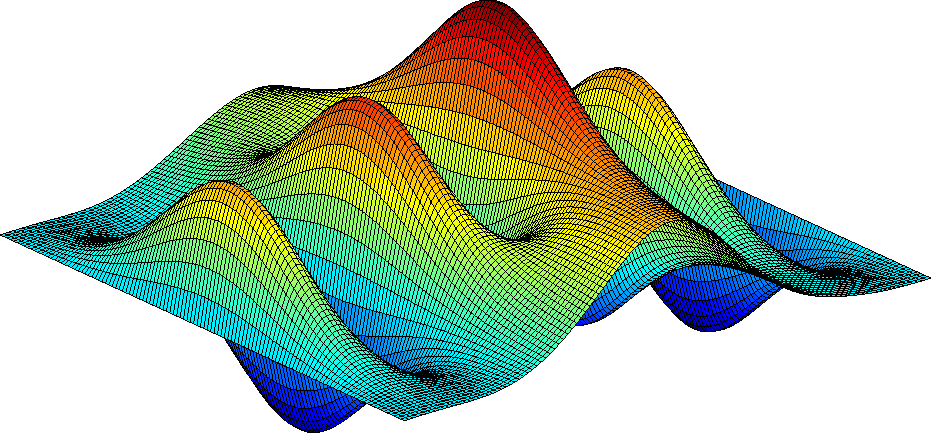
\includegraphics[width=6cm]{plotdata/plotgraphics3dsurf.png}}%
}

The key idea is now to identify several points in the image, and assign
\emph{both} their logical three-dimensional coordinates \emph{and} the
corresponding two-dimensional canvas coordinates in image coordinates. How?
Well, the three-dimensional coordinates are known to Matlab, it can display
them for you if you click somewhere into the image, compare
Figure~\ref{fig:plotgraphics3d} (left).


\begin{figure}
    \noindent
    \hbox to \linewidth{\hfill
        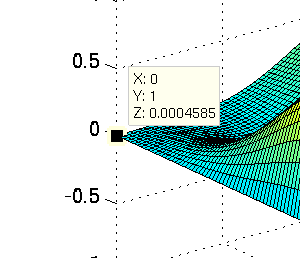
\includegraphics{plotdata/plotgraphics3dsurfmatlab.png}%
        \hfill
        \begin{minipage}[b][4cm][c]{2.6cm}%
        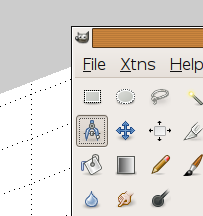
\includegraphics[width=\linewidth]{plotdata/plotgraphics_gimpmeasure.png}%
        \end{minipage}
        \hfill
    }
    \caption{Using Matlab to extract image coordinates (left) and Gimp to
             measure distances (right).}
        \label{fig:plotgraphics3d}
\end{figure}


The two-dimensional canvas coordinates need work; they need to be provided
relative to the \emph{lower left corner} of the image. I used |gimp| and
activated ``Points'' as units (lower left corner). The lower left corner now
displays the image coordinates in |pt| which is compatible with \PGFPlots{}. An
alternative to pointing onto coordinates is a measurement tool; compare
Figure~\ref{fig:plotgraphics3d} (right) for the ``Measure'' tool in |gimp|
which allows to compute the length of a line (in our case, the length of the
lower left corner to the point of interest).

I selected four points in the graphics and noted their 2d image coordinates and
their 3d logical coordinates as follows:
%
\begin{codeexample}[]
\begin{tikzpicture}
\begin{axis}[
    grid=both,minor tick num=1,
    xlabel=$x$,ylabel=$y$,
]
    \addplot3 graphics [
        points={% important
            (0,1,0) => (0,207-112)
            (1,0,0) => (446,207-133)
            (0.5546,0.5042,1.825) => (236,207)
            (0,0,0) => (194,207-202)
        },
    ] {plotdata/plotgraphics3dsurf.png};
\end{axis}
\end{tikzpicture}
\end{codeexample}
%
Here, the |points| key gets our collected coordinates as argument. It accepts a
sequence of maps of the form \meta{3d logical coordinate} | => | \meta{2d
canvas coordinate}. In our case, |(0,1,0)| has been found in the |.png| file at
|(0,207-112)|. Note that I introduced the difference since |gimp| counts from
the upper left, but \PGFPlots{} counts from the lower left.

Once these four point coordinates are gathered, we find Matlab's surface plot
in a \PGFPlots{} axis. You can modify any appearance options, including
different axis limits or further |\addplot| commands:
%
\begin{codeexample}[]
\begin{tikzpicture}
\begin{axis}[
    xmax=1.5,% extra limits
    grid=both,minor tick num=1,
    xlabel=$x$,ylabel=$y$,
]
    \addplot3 [surf] % 'surf': only used for legend
        graphics [
            points={
                (0,1,0) => (0,207-112)
                (1,0,0) => (446,207-133)
                (0.5546,0.5042,1.825) => (236,207)
                (0,0,0) => (194,207-202)
        },
    ] {plotdata/plotgraphics3dsurf.png};
        \addlegendentry{Graphics}

    \addplot3+ [only marks] coordinates {
        (0,1,0) (1,0,0)
        (0.5546,0.5042,1.825) (0,0,0)
    };
        \addlegendentry{Scatter}
\end{axis}
\end{tikzpicture}
\end{codeexample}
%
\noindent \PGFPlots{} uses the four input points to compute appropriate |x|,
|y| and |z| unit vectors (and the origin in graphics coordinates). These four
vectors (with two components each) can be computed as a result of a linear
system of size $8\times 8$, that is why you need to provide four input points
(each has two coordinates). \PGFPlots{} computes the unit vectors of the
imported graphics, and afterwards it rescales the result such that it fits into
the specified |width| and |height|. This rescaling respects the
|unit vector ratio| (more precisely, it uses |scale mode=scale uniformly|
instead of |scale mode=stretch to fill|). Consequently, the freedom to change
the view of a three-dimensional axis which contains a projected graphics is
considerably smaller than before. Surprisingly, you can still change axis
limits and |width| and |height| -- \PGFPlots{} will take care of a correct
display of your imported graphics. Since version~1.6, you can also change
|zmin| and/or |zmax| -- \PGFPlots{} will respect your changes as good as it
can.

Here is a further example. Suppose we are given the three-dimensional
visualization

{\setlength{\fboxsep}{0pt}%
\centering%
\fbox{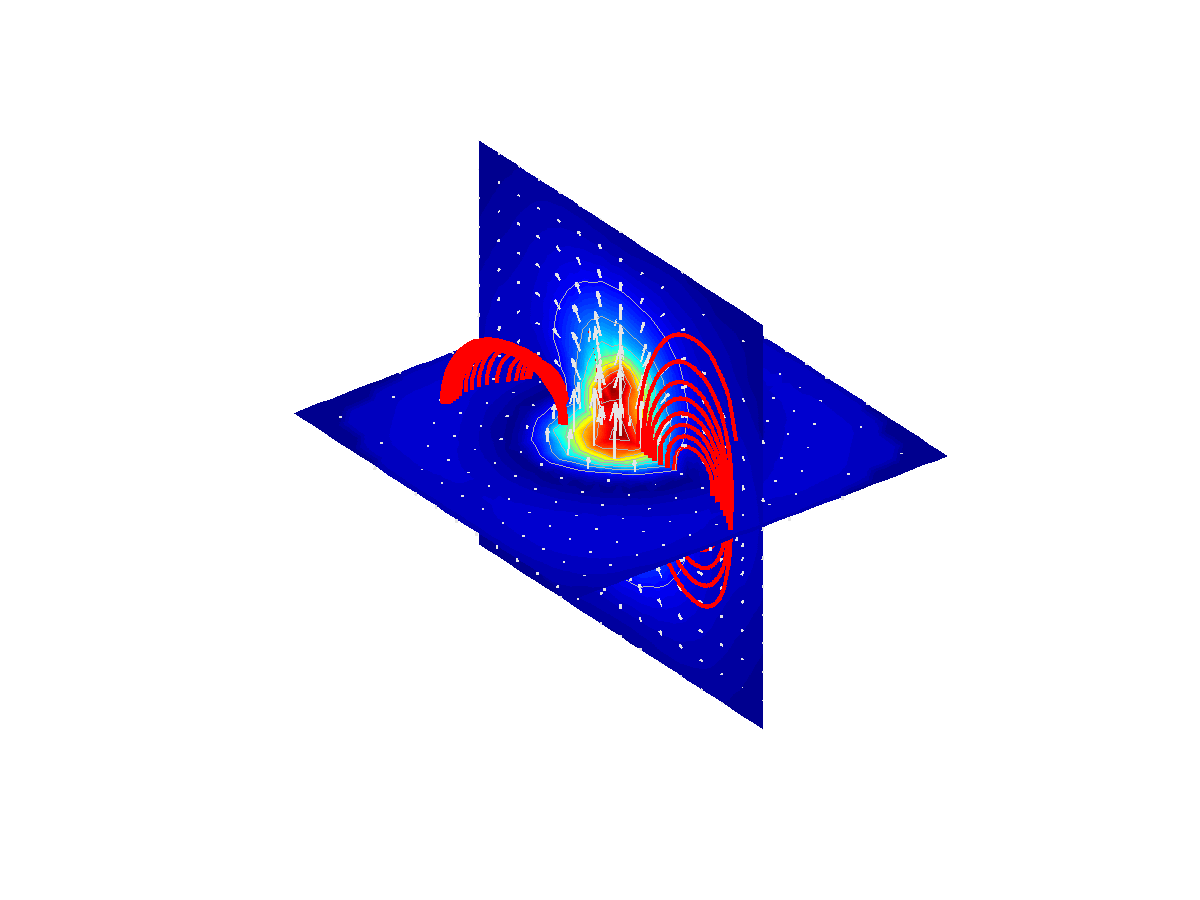
\includegraphics[width=6cm]{plotdata/risingdrop3d}}%
}

It has been generated by Matlab (I only added transparency to the background
with |gimp|). Besides advanced visualization techniques, it uses |axis equal|,
i.e.\@ |unit vector ratio=1 1 1|. As before, we need to identify four points,
each with its 3d logical coordinates (from Matlab) and the associated 2d canvas
coordinates relative to the lower left corner of the graphics (note that there
is a lot of white space around the graphics). Here is the output of \PGFPlots{}
when you import the resulting graphics:
%
\begin{codeexample}[]
\begin{tikzpicture}
\begin{axis}[
    grid=both,minor tick num=1,
    xlabel=$x$,ylabel=$y$,
    title={\centering
      Geometry provided by Sven Gro\ss, Bonn\\
      \url{http://www.igpm.rwth-aachen.de/DROPS}\\},
    title style={text width=6cm,font=\tiny},
]
    \addplot3 graphics [
        points={
            (-0.002625,0.002625,0) => (140,234)
            (0,0.00263,0.00263)    => (230,364)
            (0,-0.00263,-0.00263)  => (366,81)
            (0,-0.00263,0.00263)   => (366,276)
            (0.002625,0.002625,0.002625)
        },
    ] {plotdata/risingdrop3d.png};
\end{axis}
\end{tikzpicture}
\end{codeexample}
%
\noindent Note that I provided \emph{five} three-dimensional coordinates here,
but the last entry has no |=>| mapping to two-dimensional canvas coordinates.
Thus, it is only used to update the bounding box (see the reference manual for
the |points| key for details).

The example above leads to a relatively small image and much ``empty space''.
This is due to the |scale mode=scale uniformly| implementation of \PGFPlots{}:
it decided that the best way is to enlarge the involved axis limits. Here,
``best way'' means to satisfy |width|/|height| constraints combined with
minimally enlarged (never shrinked) axis limits. The remaining degrees of
freedom are |width|, |height|, and the axis limits. In our case, changing the
ratio between |width| and |height| improves the display:

\begin{codeexample}[]
\begin{tikzpicture}
\begin{axis}[
    height=8cm,width=7cm,% improve scaling manually
    grid=both,minor tick num=1,
    xlabel=$x$,ylabel=$y$,
    title={\centering
      Geometry provided by Sven Gro\ss, Bonn\\
      \url{http://www.igpm.rwth-aachen.de/DROPS}\\},
    title style={text width=6cm,font=\tiny},
]
    \addplot3 graphics [
        points={
            (-0.002625,0.002625,0) => (140,234)
            (0,0.00263,0.00263)    => (230,364)
            (0,-0.00263,-0.00263)  => (366,81)
            (0,-0.00263,0.00263)   => (366,276)
            (0.002625,0.002625,0.002625)
        },
    ] {plotdata/risingdrop3d.png};
\end{axis}
\end{tikzpicture}
\end{codeexample}
%
\noindent What happens is that \PGFPlots{} selects a \emph{single} scaling
factor which is applied to all units as they have been deduced from the
|points| key. This ensures that the imported graphics fits correctly into the
axis. In addition, \PGFPlots{} does its best to satisfy the remaining
constraints.

The complete description of how \PGFPlots{} scales the axis can be found in the
documentation for |scale mode=scale uniformly|. Here is just a brief summary:
\PGFPlots{} assumes that the prescribed |width| and |height| have to be
satisfied. To this end, it rescales the projected unit vectors (i.e.\@ the
space which is taken up for each unit in $x$, $y$, and $z$) and it can modify
the axis limits. In the default configuration |scale uniformly strategy=auto|,
\PGFPlots{} will \emph{never} shrink axis limits.


\paragraph{Compatibility remark:}

Note that the scaling capabilities have been improved for \PGFPlots{}
version~1.6. In previous versions, only
|scale uniformly strategy=change vertical limits| was available which lead to
clipped axes. In short: please consider writing |\pgfplotsset{compat=1.6}| or
newer into your document to benefit from the improved scaling. If you have
|\pgfplotsset{compat=1.5}| or older, the outcome for |\addplot3 graphics| will
be different.

We consider a third example which has been generated by the Matlab code
%
\begin{codeexample}[code only]
clear all
close all
seed = sum(clock)
rand('seed',seed);
X = rand(10,10,10);
data = smooth3(X,'box',5);
p1 = patch(isosurface(data,.5), ...
   'FaceColor','blue','EdgeColor','none');
p2 = patch(isocaps(data,.5), ...
    'FaceColor','interp','EdgeColor','none');
isonormals(data,p1)
daspect([1 2 2])
view(3); axis vis3d tight
camlight; lighting phong
% print -dpng plotgraphics3withaxis
axis off
print -dpng plotgraphics3
save  plotgraphics3.seed seed -ASCII % to reproduce the result
\end{codeexample}
%
\noindent I only added background transparency with |gimp| and got the following
graphics:

{\setlength{\fboxsep}{0pt}%
\centering%
\fbox{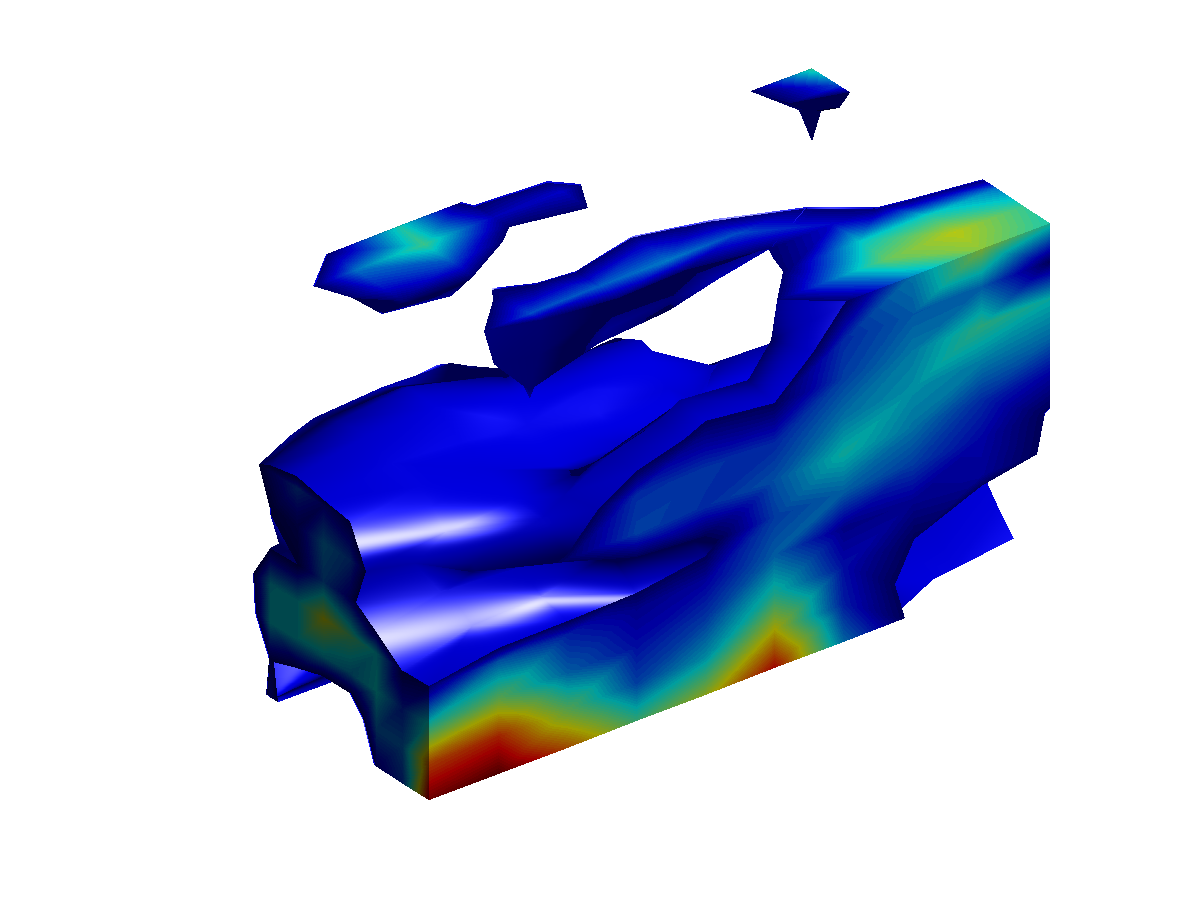
\includegraphics[width=6cm]{plotdata/plotgraphics3.png}}%
}

We proceed as before and collect four points, each with 3d logical coordinates
(by clicking into the Matlab figure) and their associated 2d canvas (graphics)
coordinates using the measure tool of gimp. The result is shown in the code
example below.
%
\begin{codeexample}[]
\begin{tikzpicture}
\begin{axis}[
    grid=both,minor tick num=1,
    xlabel=$x$,ylabel=$y$,
    3d box,
]
    \addplot3 graphics [
        points={
            (1,1,1)    => (205,48)
            (10,1,10)  => (503,324)
            (1,1,4.044)=> (206,102)
            (10,10,10) => (390,398)
        },
    ] {plotdata/plotgraphics3.png};
\end{axis}
\end{tikzpicture}
\end{codeexample}
%
\noindent Note that it has non-standard data aspect ratio which is respected by
\PGFPlots{} automatically.


\subsection*{External Three-Dimensional Graphics and Matlab}
\label{sec:plotgraphics3d:matlabscript}

\textit{An extension by Jürnjakob Dugge} \vskip\baselineskip

\noindent The procedure to map three-dimensional logical coordinates to
two-dimensional canvas coordinates is tedious.

Jürnjakob Dugge contributed a script which does most of the logic and your work
is reduced to a copy--paste job. With his permission, I post the contribution
here.

The idea is to start a simple script which \emph{records} mappings for any
coordinates which have been clicked by the user. It works as follows:
%
\begin{enumerate}
    \item Create the Matlab plot, say, using
        %
\begin{codeexample}[code only]
hist3(randn(10000,2)) % some random data
set(get(gca,'child'),'FaceColor','interp','CDataMode','auto'); % colors
% make sure the "print" paper format is the same as the screen paper format:
set(gcf,'PaperPositionMode','auto')
\end{codeexample}
        %
    \item Save the following code as |pgfplotscsconversion.m|:
        %
\begin{codeexample}[code only]
function pgfplotscsconversion

% Hook into the Data Cursor "click" event
h = datacursormode(gcf);
set(h,'UpdateFcn',@myupdatefcn,'SnapToDataVertex','off');
datacursormode on

% select four points in plot using mouse

% The function that gets called on each Data Cursor click
function [txt] = myupdatefcn(obj,event_obj)

% Get the screen resolution, in dots per inch
dpi = get(0,'ScreenPixelsPerInch');

% Get the click position in pixels, relative to the lower left of the
% screen
screen_location=get(0,'PointerLocation');

% Get the position of the plot window, relative to the lower left of
% the screen
figurePos = get(gcf,'Position');

% Get the data coordinates of the cursor
pos = get(event_obj,'Position');

% Format the data and figure coordinates. The factor "72.27/dpi" is
% necessary to convert from pixels to TeX points (72.27 poins per inch)
display(['(',num2str(pos(1)),',',num2str(pos(2)),',',num2str(pos(3)),') => (', ...
   num2str((screen_location(1)-figurePos(1))*72.27/dpi),',', ...
   num2str((screen_location(2)-figurePos(2))*72.27/dpi),')'])

% Format the tooltip display
txt = {['X: ',num2str(pos(1))],['Y: ',num2str(pos(2))],['Z: ',num2str(pos(3))]};
\end{codeexample}
        %
        Run |pgfplotscsconversion|, click on four points in your plot.
        Preferably select non-colinear points near the edges of the plot. Copy
        and paste the four lines that were written to the Matlab command
        window.

        Make sure that the first two points have different $X$ and $Y$ values
        on screen (i.e.\@ image canvas coordinates).
    \item Export the plot as an image
        %
\begin{codeexample}[code only]
axis off
print -dpng matlabout -r400 % PNG called "matlabout.png" with 400 dpi resolution
\end{codeexample}

        If you want to export vectors graphics, you should note that |pdf|
        output of Matlab is clumsy. It might be best to export to |eps| first,
        followed by a conversion from |eps| to |pdf|.

        \emph{If} you really want to use |pdf| output of Matlab, you may need
        to set the paper size to match the figure size by yourself, since the
        PDF driver does not automatically adjust the size:
        %
\begin{codeexample}[code only]
% It might be better to use print -depsc followed by epstopdf.
% Use this if you (really) want to use print -dpdf:
currentScreenUnits=get(gcf,'Units')     % Get current screen units
currentPaperUnits=get(gcf,'PaperUnits') % Get current paper units
set(gcf,'Units',currentPaperUnits)      % Set screen units to paper units
plotPosition=get(gcf,'Position')        % Get the figure position and size
set(gcf,'PaperSize',plotPosition(3:4))  % Set the paper size to the figure size
set(gcf,'Units',currentScreenUnits)     % Restore the screen units

print -dpdf matlabout      % PDF called "matlabout.pdf"
\end{codeexample}
        %
    \item Include the image in your \PGFPlots{} axis. If you selected points
        on the plot corners, your |xmin|, |xmax|, |ymin| and |ymax| should be
        set automatically, otherwise you may want to provide those yourself.
        Also, adjustments of |width| and |height| might be of interest to get
        the right vertical placement of the plot. Consider changing |zmin|
        and/or |zmax| to fit your needs (preferably only one of them;
        otherwise \PGFPlots{} may be unable to fix the |height|).
\end{enumerate}

This contribution is from

\noindent
\url{http://tex.stackexchange.com/questions/52987/3-dimensional-histogram-in-pgfplots} .


\subsection*{Summary: External Three-Dimensional Graphics}

As has been shown in the previous sections, \verbpdfref{\addplot3} |graphics|
allows to include three-dimensional graphics and \PGFPlots{} overlays a
flexible axis with all its power. The cost to do so is
%
\begin{enumerate}
    \item collect both logical three-dimensional coordinates \emph{and}
        image-internal two-dimensional coordinates for \emph{four points} of
        your graphics.

        In Matlab, this can be simplified by the tool mentioned on
        page~\pageref{sec:plotgraphics3d:matlabscript}.
    \item If your axes form a right-handed coordinate system, that is all. If
        not, also add |x dir=reverse| for any reversed axes.
\end{enumerate}

\noindent Consider the following list of you encounter problems while working
with \verbpdfref{\addplot3} |graphics|:
%
\begin{itemize}
    \item It must be possible to deduce the origin and the three
        (two-dimensional) unit vectors from the four provide |points|;
        otherwise the algorithm will fail.

        The algorithm should detect any deficiencies. However, if you
        encounter strange ``Dimension too large'' messages here, you can try
        other arguments in |points|. Take a look into your logfile, it will
        probably indicate the source of problems (or use the |debug| key).
    \item Ensure that the external graphics has an orthogonal axis. In fact,
        the axis may be skewed (just like a \PGFPlots{} axis can be created
        by means of custom |x|, |y|, and |z| vectors). However, the external
        image must not have perspective projection as this is unsupported by
        \PGFPlots{}. The |points| command needs to receive four points which
        belong to linearly independent position vectors.
    \item \PGFPlots{} uses the first two points to squeeze the graphics into
        the desired coordinates (which implies that they should not have the
        same canvas $X$ or $Y$ coordinates). It verifies that the remaining
        |points| arguments are projected correctly.
    \item The resulting scaling by means of |scale mode=scale uniformly| will
        try to satisfy all scaling constraints. You can change these
        constraints by modifying |width|, |height|, |xmin|, |xmax|, |ymin|,
        |ymax|, |zmin|, |zmax| and/or any combination of these parameters.
        See also |unit rescale keep size| which controls the flexibility of
        limit changes. There is also a key |scale uniformly strategy| which
        allows to select a different scaling strategy.
    \item The image should have a ``right-handed coordinate system'': you
        should be able to take your right hand, point your thumb in direction
        of the $x$-axis, your first finger in direction of~$y$, and your
        second finger in direction of the $z$-axis. If that is impossible,
        once of your axes is reversed and you need to communicate that to
        \PGFPlots{} explicitly by means of the |x dir=reverse| key (and its
        variants).
    \item Note that this feature has been verified with standard Cartesian
        axes only.
    \item There is a |debug| key to investigate what the algorithm is doing:
        %
        \begin{pgfplotskey}{plot graphics/debug=\mchoice{true,false,visual} (initially false)}
            If you provide |\addplot3 graphics[debug,points={...}]|,
            \PGFPlots{} will provide debug information onto your terminal and
            into the logfile. It will also generate extra files containing the
            determined unit vectors and the linear system used to derive them
            (one such file for every |\addplot3 graphics| statement, the
            filename will be the graphics file name and |.dat| appended).

            Without the |debug| key, only the logfile will contain brief
            information what \PGFPlots{} is doing behind the scenes.

            The choice \declaretext{true} activates log messages. The choice
            \declaretext{visual} activates log messages \emph{and} places some
            filled circles at the provided |points|. The choice
            \declaretext{false} disables all |debug| features.
        \end{pgfplotskey}
\end{itemize}
}


\subsection{Reading Coordinates From Files}

\begin{addplotoperation}[]{file}{\marg{name}}
\label{pgfplots:addplot:file}

    \paragraph{Deprecation note:}

    If you have data files, you should generally use |\addplot table|. The
    input type |\addplot file| is almost the same, but considerably less
    powerful. It is only kept for backwards compatibility.

    The |\addplot file| input mechanism is similar to the \Tikz{} command
    `|\addplot file|'. It is to be used like

\begin{codeexample}[code only]
\addplot file {datafile.dat};
\end{codeexample}
    %
    where \meta{name} is a text file with at least two columns which will be
    used as $x$- and $y$-coordinates. Lines starting with `|%|' or `|#|' are
    ignored. Such files are often generated by \textsc{gnuplot}:
    %
\begin{codeexample}[code only]
#Curve 0, 20 points
#x y type
0.00000 0.00000 i
0.52632 0.50235 i
1.05263 0.86873 i
1.57895 0.99997 i
...
9.47368 -0.04889 i
10.00000 -0.54402 i
\end{codeexample}
    %
    This listing has been copied from~\cite[Section~16.4]{tikz}.

    Plot file accepts one optional argument,

\begin{codeexample}[code only]
\addplot file [skip first] {datafile.dat};
\end{codeexample}

    \noindent which allows to skip over a non-comment header line. This allows
    to read the same input files as |\addplot table| by skipping over column names.
    Please note that comment lines do not count as lines here.

    The input method |\addplot file| can also read meta data for every coordinate.
    As already explained for |\addplot coordinates| (see above), meta data can be
    used to change colors or other style parameters for every marker
    separately. Now, if |point meta| is set to |explicit| or to
    |explicit symbolic| and the input method is |\addplot file|, one further element
    will be read from disk -- for every line. Meta data is always the last
    element which is read. See page~\pageref{pgfplots:scatter:src} for
    information and examples about per point meta data and
    page~\pageref{pgfplots:scatterclasses} for an application example using
    |scatter/classes|.

    Plot file is very similar to |\addplot table|: you can achieve the same effect
    with
    %
\begin{codeexample}[code only]
\addplot table [x index=0,y index=1,header=false] {datafile.dat};
\end{codeexample}
    %
    \noindent Due to its simplicity, |\addplot file| is slightly faster while
    |\addplot table| allows higher flexibility.

    Technical note: every opened file will be protocolled into your logfile.

    The file can contain |empty line|s to tell \PGFPlots{} that the function
    has jumps. To use it, simply insert an empty line (and ensure that you have
    |\pgfplotsset{compat=1.4}| or newer in your preamble). See the
    documentation of |empty line| for details.
\end{addplotoperation}

\begin{pgfplotskeylist}{%
    plot file/skip first=\mchoice{true,false} (initially false),
    plot file/ignore first=\mchoice{true,false} (initially false)%
}
    The two keys can be provided as arguments to
    |\addplot file[|\meta{options}|] |\marg{filename}|;| to skip the first
    non-comment entry in the file. They are equivalent. If you provide them in
    this context, the prefix |/pgfplots/plot file| can be omitted.
\end{pgfplotskeylist}
}
